\begin{enumerate}[label=\thesection.\arabic*,ref=\thesection.\theenumi]
\numberwithin{equation}{enumi}
\numberwithin{figure}{enumi}
\numberwithin{table}{enumi}
\item Check whether$(5,-2),(6,4)$ and $(7,-2)$ are the vertices of an isosceles triangle.
\item Name the type of quadrilateral formed, if any, by the following points,and give reasons for your answer
\begin{enumerate}
\item $(-1,-2),(1,0),(-1,2),(-3,0)$
\item $(-3,5),(-3,1),(0,3),(-1,-4)$
\item $(4,5),(7,6),(4,3),(1,2)$
\end{enumerate}
\solution
		\iffalse
\documentclass[12pt]{article}
\usepackage{graphicx}
\usepackage{amsmath}
\usepackage{mathtools}
\usepackage{gensymb}

\newcommand{\mydet}[1]{\ensuremath{\begin{vmatrix}#1\end{vmatrix}}}
\providecommand{\brak}[1]{\ensuremath{\left(#1\right)}}
\providecommand{\norm}[1]{\left\lVert#1\right\rVert}
\newcommand{\solution}{\noindent \textbf{Solution: }}
\newcommand{\myvec}[1]{\ensuremath{\begin{pmatrix}#1\end{pmatrix}}}
\let\vec\mathbf

\begin{document}
\begin{center}
\textbf\large{CHAPTER-7 \\ COORDINATE GEOMETRY}

\end{center}
\section*{Excercise 7.1}

Q6.Name the type of quadilateral formed,if any, by the following points, and give reasons for your answer:
\begin{enumerate}
	\item $\brak{-1,-2}, \brak{1,0}, \brak{-1,2}, \brak{-3,0}$ 
	\item $\brak{-3,5}, \brak{3,1}, \brak{0,3}, \brak{-1,-4}$
	\item $\brak{4,5}, \brak{7,6}, \brak{4,3}, \brak{1,2}$
\end{enumerate}
\solution
\fi
\begin{enumerate}
\item The coordinates are given as
	\begin{align}
	\vec{A} = \myvec{
		-1\\
		-2\\
		},
	\vec{B} = \myvec{
		1\\
		0\\
		},
	\vec{C} = \myvec{
		-1\\
		2\\
		} \text{ and }
	\vec{D} = \myvec{
		-3\\
		0\\
		}
	\end{align}
	\begin{align}
		\vec{B} - \vec{A} &= \myvec{1\\0} - \myvec{-1\\-2} = \myvec{2\\2}\\
		\vec{C} - \vec{B} &= \myvec{-1\\2} - \myvec{1\\0} = \myvec{-2\\2}\\
		\vec{C} - \vec{D} &= \myvec{-1\\2} - \myvec{-3\\0} = \myvec{2\\2}\\
		\vec{D} - \vec{A} &= \myvec{-3\\0} - \myvec{-1\\-2} = \myvec{-2\\2}
	\end{align}
	\begin{align}	
		\vec{C} - \vec{A} &= \myvec{-1\\2} - \myvec{-1\\-2} = \myvec{0\\4}\\
		\vec{D} - \vec{B} &= \myvec{-3\\0} - \myvec{1\\0} = \myvec{-4\\0}
	\end{align}
	\begin{align}	
		\vec{B}-\vec{A} = \vec{C}-\vec{D} \text{ and } \vec{C}-\vec{B} = \vec{D}-\vec{A}.
	\end{align}
	Hence, $ABCD$ is a parallelogram.
	\begin{enumerate}
		\item Now checking if the adjacent sides are orthogonal to each other
	\begin{align}
		(\vec{B}-\vec{A})^\top (\vec{C}-\vec{B}) = \myvec{2&2} \myvec{-2\\2} = -4+4 = 0
	\end{align}
		\item Now checking if the diagonals are also orthogonal then it is a square else a rectangle.
	\end{enumerate}	
	\begin{align}
		(\vec{C}-\vec{A})^\top (\vec{D}-\vec{B}) = \myvec{0&4} \myvec{-4\\0} = 0
	\end{align}
	Hence the diagonals are orthogonal to each other.

	So, we can conclude that $ABCD$ is a square.

	As shown in Figure \ref{fig:10/7/1/6/Fig1} we can see that $ABCD$ is a square hence we can conclude that our theoritical result is verified.
 
\begin{figure}[!h]
	\begin{center} 
	    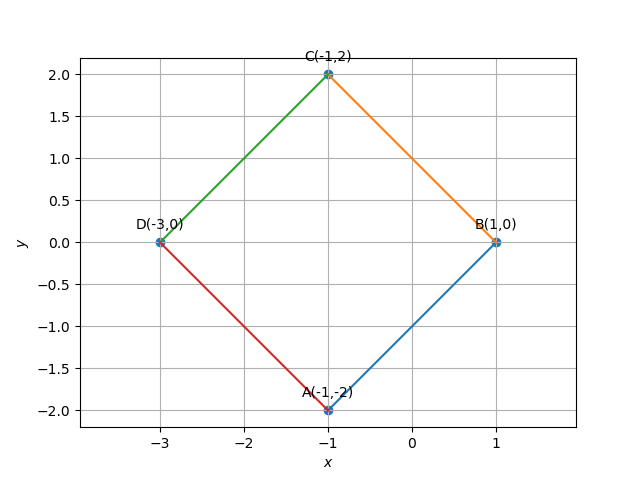
\includegraphics[width=\columnwidth]{chapters/10/7/1/6/figs/quad1}
	\end{center}
\caption{}
\label{fig:10/7/1/6/Fig1}
\end{figure}

\item The coordinates are given as
	\begin{align}
	\vec{A} = \myvec{
		-3\\
		5\\
		},
	\vec{B} = \myvec{
		3\\
		1\\
		},
	\vec{C} = \myvec{
		0\\
		3\\
		} \text{ and }
	\vec{D} = \myvec{
		-1\\
		-4\\
		}
	\end{align}
	\begin{align}
		\vec{B} - \vec{A} &= \myvec{3\\1} - \myvec{-3\\5} = \myvec{6\\-4}\\
		\vec{C} - \vec{B} &= \myvec{0\\3} - \myvec{3\\1} = \myvec{-3\\2}\\
		\vec{C} - \vec{D} &= \myvec{0\\3} - \myvec{-1\\-4} = \myvec{1\\7}\\
		\vec{D} - \vec{A} &= \myvec{-1\\-4} - \myvec{-3\\5} = \myvec{2\\-9}
	\end{align}
	\begin{align}
		\vec{C} - \vec{A} &= \myvec{0\\3} - \myvec{-3\\5} = \myvec{3\\-2}\\
		\vec{D} - \vec{B} &= \myvec{-1\\-4} - \myvec{3\\1} = \myvec{-4\\-5}
	\end{align}
	\begin{align}
	\vec{B}-\vec{A} \neq \vec{C}-\vec{D} \text{ and } \vec{C}-\vec{B} \neq \vec{D}-\vec{A},
	\end{align}
	Hence, $ABCD$ is not a parallelogram, it can be a irregular quadilateral.
	\begin{enumerate}
		\item Now to check if any three points are collinear,

	if rank of $\myvec{\vec{B}-\vec{A} & \vec{C}-\vec{B}} = 1$ then points are collinear

	Forming the collinearity matrix
	\begin{align}
		\myvec{6&-3\\-4&2} \xleftrightarrow{R_{2}\rightarrow R_{2}+\frac{2}{3}R_{1}}= \myvec{6&-3\\0&0}
	\end{align}
	\end{enumerate}
	Hence, rank = 1

	Since none of the opposite sides are parallel to each other and three points are collinear so these does not form a quadilateral.

	As shown in Figure \ref{fig:10/7/1/6/Fig2} we can see that $ABCD$ does not form a quadilateral and three points are collinear hence, our theoritical result is verified.
	
\begin{figure}[!h]
	\begin{center} 
	    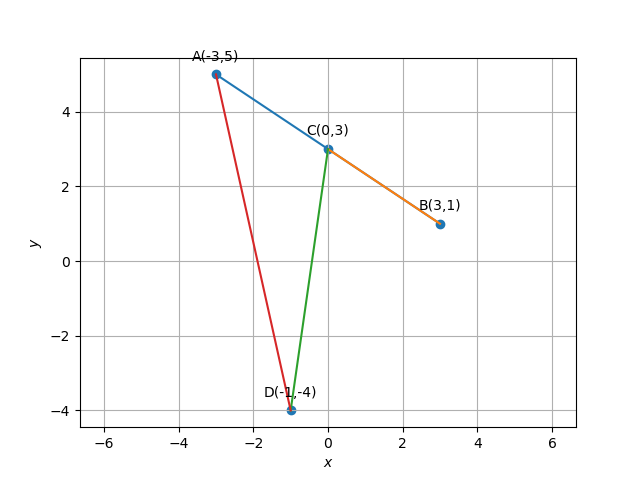
\includegraphics[width=\columnwidth]{chapters/10/7/1/6/figs/quad2}
	\end{center}
\caption{}
\label{fig:10/7/1/6/Fig2}
\end{figure}
	
\item The coordinates are given as
	\begin{align}
	\vec{A} = \myvec{
		4\\
		5\\
		},
	\vec{B} = \myvec{
		7\\
		6\\
		},
	\vec{C} = \myvec{
		4\\
		3\\
		} \text{ and }
	\vec{D} = \myvec{
		1\\
		2\\
		}
	\end{align}
	\begin{align}
		\vec{B} - \vec{A} &= \myvec{7\\6} - \myvec{4\\5} = \myvec{3\\1}\\
		\vec{C} - \vec{B} &= \myvec{4\\3} - \myvec{7\\6} = \myvec{-3\\-3}\\
		\vec{C} - \vec{D} &= \myvec{4\\3} - \myvec{1\\2} = \myvec{3\\1}\\
		\vec{D} - \vec{A} &= \myvec{1\\2} - \myvec{4\\5} = \myvec{-3\\-3}
	\end{align}
	\begin{align}
		\vec{C} - \vec{A} &= \myvec{4\\3} - \myvec{4\\5} = \myvec{0\\-2}\\
		\vec{D} - \vec{B} &= \myvec{1\\2} - \myvec{7\\6} = \myvec{-6\\-4}
	\end{align}
	\begin{align}
		\vec{B}-\vec{A} = \vec{C}-\vec{D} \text{ and } \vec{C}-\vec{B} = \vec{D}-\vec{A},
	\end{align}
	Hence, $ABCD$ is a parallelogram.
	\begin{enumerate}
		\item Now checking if the adjacent sides are orthogonal to each other
	\begin{align}
		(\vec{B}-\vec{A})^\top (\vec{C}-\vec{B}) = \myvec{3&1} \myvec{-3\\-3} = -9-3 = -12
	\end{align}
	Since inner product is not zero so adjacent sides are not orthogonal.

	Hence, we can say that $ABCD$ is neither a rectangle nor a square.

		\item Now checking if the diagonals are orthogonal then it is a Rhombus.
	\begin{align}
		(\vec{C}- \vec{A})^\top (\vec{D}-\vec{B}) = \myvec{0&-2} \myvec{-6\\-4} = 0+8 = 8
	\end{align}
	\end{enumerate}		
	Hence the diagonals are also not orthogonal so we conclude that $ABCD$ is a parallelogram.

	As shown in Figure \ref{fig:10/7/1/6/Fig3} we can see that $ABCD$ forms a parallelogram hence, our theoritical result is verified.

\begin{figure}[!h]
	\begin{center} 
	    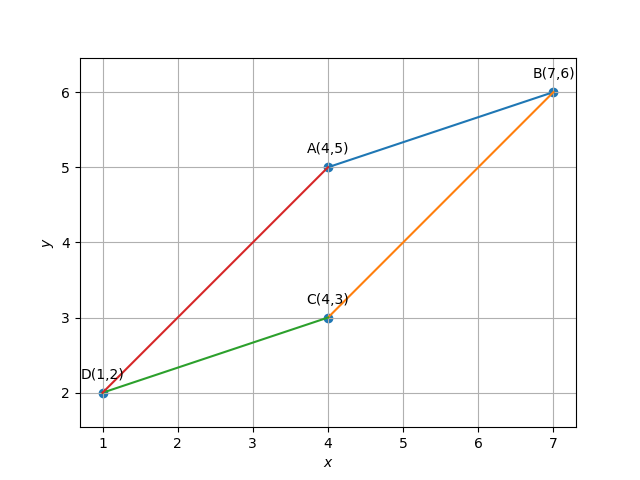
\includegraphics[width=\columnwidth]{chapters/10/7/1/6/figs/quad3}
	\end{center}
\caption{}
\label{fig:10/7/1/6/Fig3}
\end{figure}
\end{enumerate}



\item Find the projection of the vector $\hat{i}-\hat{j}$ on the vector $\hat{i}+\hat{j}$.
	\\
		\iffalse
\documentclass[12pt]{chapters/10/7/4/3/figsarticle}
\usepackage{graphicx}
\usepackage[none]{chapters/10/7/4/3/figshyphenat}
\usepackage{graphicx}
\usepackage{listings}
\usepackage[english]{chapters/10/7/4/3/figsbabel}
\usepackage{graphicx}
\usepackage{caption} 
\usepackage{booktabs}
\usepackage{array}
\usepackage{amssymb} % for \because
\usepackage{amsmath}   % for having text in math mode
\usepackage{extarrows} % for Row operations arrows
\usepackage{listings}
\lstset{
  frame=single,
  breaklines=true
}
\usepackage{hyperref}
  
%Following 2 lines were added to remove the blank page at the beginning
\usepackage{atbegshi}% http://ctan.org/pkg/atbegshi
\AtBeginDocument{\AtBeginShipoutNext{\AtBeginShipoutDiscard}}


%New macro definitions
\newcommand{\mydet}[1]{chapters/10/7/4/3/figs\ensuremath{\begin{vmatrix}#1\end{vmatrix}}}
\providecommand{\brak}[1]{chapters/10/7/4/3/figs\ensuremath{\left(#1\right)}}
\newcommand{\solution}{\noindent \textbf{Solution: }}
\newcommand{\myvec}[1]{chapters/10/7/4/3/figs\ensuremath{\begin{pmatrix}#1\end{pmatrix}}}
\providecommand{\norm}[1]{chapters/10/7/4/3/figs\left\lVert#1\right\rVert}
\providecommand{\abs}[1]{chapters/10/7/4/3/figs\left\vert#1\right\vert}
\let\vec\mathbf


\begin{document}

\begin{center}
\title{\textbf{VECTORS}}
\date{\vspace{-5ex}} %Not to print date automatically
\maketitle
\end{center}

\setcounter{page}{1}

\section{10$^{th}$ Maths - Chapter 10}

This is Problem-3 from Exercise 10.3

\begin{enumerate}
\item Find the projection of the vector $\hat{i}-\hat{j}$ on the vector $\hat{i}+\hat{j}$  
\end{enumerate}
\section{SOLUTION}
\fi
\solution
The given points are
\begin{align}
 \vec{A}=\myvec{1\\ -1},
 \vec{B}=\myvec{1\\ 1}
\end{align}
Since
\begin{align}
	\vec{A}^\top \vec{B} &= \myvec{1 &-1} \myvec{1\\ 1}=\myvec{1 \times 1}+\myvec{-1 \times  1}=0
	\\
	\norm {\vec {B}}^2 &= (\vec{B}^\top  \vec{B})=\myvec{1 & 1} \myvec{1\\ 1}= (1 \times  1)+(1 \times  1)=2,
\end{align}
and the project vector is given by 
\begin{align}
	\vec{C} &= 
	\frac{\vec{A}^\top  \vec{B}}{\norm {\vec{B}}}^2 \vec{B}
	&=\frac{0}{2} \myvec{1\\ 1}
	=\myvec{0\\ 0}
\end{align}
This is verfied in Fig.
		\ref{fig:12/10/3/3Figure}.
\begin{figure}[h]
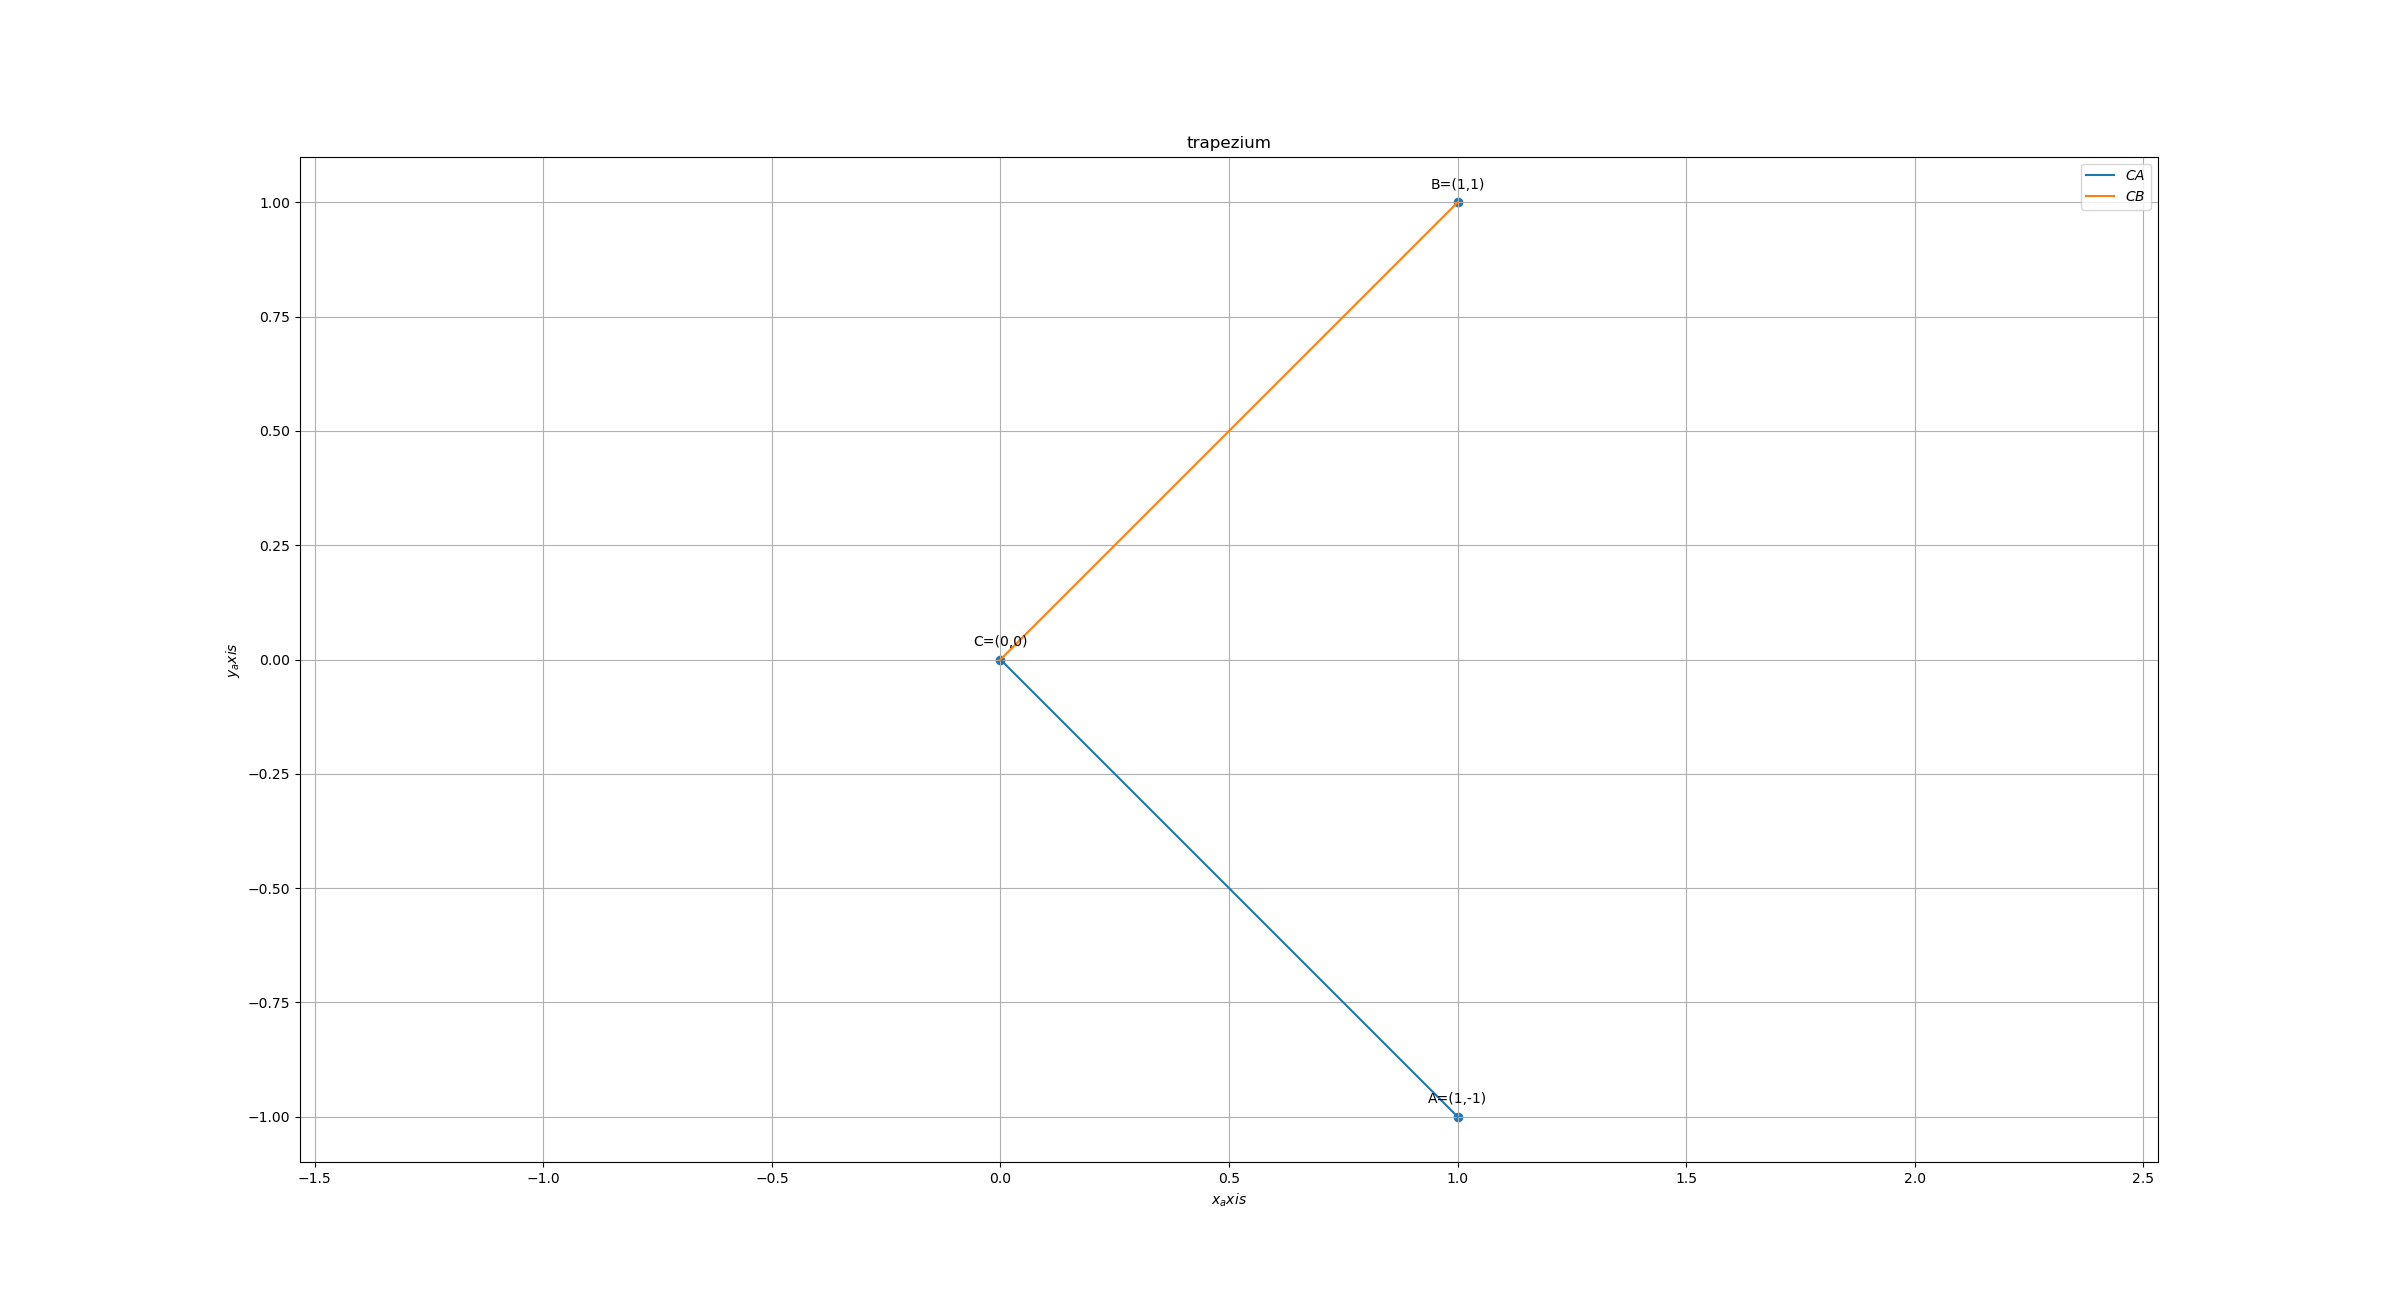
\includegraphics[width=\columnwidth]{chapters/12/10/3/3/figs/vector.png}
\caption{}
		\label{fig:12/10/3/3Figure}
\end{figure}

\item Find the projection of the vector $\hat{i}+3\hat{j}+7\hat{k}$ on the vector $7\hat{i}-\hat{j}+8\hat{k}$.
	\\
	\solution
		\iffalse
\documentclass[12pt]{article}
\usepackage{graphicx}
%\documentclass[journal,12pt,twocolumn]{IEEEtran}
\usepackage[none]{hyphenat}
\usepackage{graphicx}
\usepackage{listings}
\usepackage[english]{babel}
\usepackage{graphicx}
\usepackage{caption}
\usepackage[parfill]{parskip}
\usepackage{hyperref}
\usepackage{booktabs}
\usepackage{amsmath}
%\usepackage{setspace}\doublespacing\pagestyle{plain}
\def\inputGnumericTable{}
\usepackage{color}                                            %%
    \usepackage{array}                                            %%
    \usepackage{longtable}                                        %%
    \usepackage{calc}                                             %%
    \usepackage{multirow}                                         %%
    \usepackage{hhline}                                           %%
    \usepackage{ifthen}
\usepackage{array}
\usepackage{amsmath}   % for having text in math mode
\usepackage{parallel,enumitem}
\usepackage{listings}
\lstset{
language=tex,
frame=single,
breaklines=true
}
 
%Following 2 lines were added to remove the blank page at the beginning
\usepackage{atbegshi}% http://ctan.org/pkg/atbegshi
\AtBeginDocument{\AtBeginShipoutNext{\AtBeginShipoutDiscard}}
%
%New macro definitions
\newcommand{\mydet}[1]{\ensuremath{\begin{vmatrix}#1\end{vmatrix}}}
\providecommand{\brak}[1]{\ensuremath{\left(#1\right)}}
\providecommand{\norm}[1]{\left\lVert#1\right\rVert}
\newcommand{\solution}{\noindent \textbf{Solution: }}
\newcommand{\myvec}[1]{\ensuremath{\begin{pmatrix}#1\end{pmatrix}}}
\let\vec\mathbf
\begin{document}
\begin{center}
\enlargethispage{-4cm}
\title{\textbf{VECTOR ALGEBRA}}
\date{\vspace{-5ex}} %Not to print date automatically
\maketitle
\end{center}
\setcounter{page}{1}
\section*{12$^{th}$ Maths - Chapter 10}
This is Problem-4 from Exercise 10.3
\begin{enumerate}
	\item Find the projection of the vector $\hat{i}+3\hat{j}+7\hat{k}$ on the vector $7\hat{i}-\hat{j}+8\hat{k}$.

\solution 
\fi
		Let 
\begin{align}
 \vec{A} =\myvec{1\\3\\7}, \vec{B} =\myvec{7\\-1\\8}
\end{align}
The desired projection  is given by
\begin{align}
	\vec{C}=\frac{\Vec{A}^\top \Vec{B}}{\norm{\vec{B}}^2}\vec{B}\label{eq:chapters/12/10/3/4/2}
	  =\frac{\myvec{1 & 3 & 7}\myvec{7\\-1\\8}}{2}\myvec{7\\-1\\8}
		=\frac{10}{19}\myvec{7\\-1\\8}
 \end{align}

\item Show that each of the given three vectors is a unit vector: 
 $\frac{1}{7}(2\hat{i}+3\hat{j}+6\hat{k}),\frac{1}{7}(3\hat{i}-6\hat{j}+2\hat{k}),\frac{1}{7}(6\hat{i}+2\hat{j}-3\hat{k}$)
Also,show that they are mutually perpendicular to each other.
	\\
	\solution
		\iffalse
\documentclass[journal,12pt,twocolumn]{IEEEtran}
\usepackage{graphicx}
\graphicspath{{./figs/}}{}
\usepackage{amsmath,amssymb,amsfonts,amsthm}
\newcommand{\myvec}[1]{\ensuremath{\begin{pmatrix}#1\end{pmatrix}}}
\providecommand{\norm}[1]{\lVert#1\rVert}
\usepackage{listings}
\usepackage{watermark}
\usepackage{titlesec}
\usepackage{caption}
\let\vec\mathbf
\lstset{
frame=single, 
breaklines=true,
columns=fullflexible
}
\thiswatermark{\centering \put(0,-105.0){
\includegraphics[scale=0.15]{/sdcard/IITH/vectors/12.10.3.5/figs/logo.png}} }
\title{\mytitle}
\title{
Assignment - 12.10.3.5
}
\author{Surajit Sarkar}
\begin{document}
\maketitle
\tableofcontents
\bigskip
\section{\textbf{Problem}}
Show that each of the given three vectors is a unit vector:$\frac{1}{7}\myvec{2\hat{i}+3\hat{j}+6\hat{k}},\frac{1}{7}\myvec{3\hat{i}-6\hat{j}+2\hat{k}},\frac{1}{7}\myvec{6\hat{i}+2\hat{j}-3\hat{k}}$
Also, Show that they are mutually perpendicular to eatch other.
\section{\textbf{Solution}}
\fi
Let
\begin{align}
\vec{A}=\myvec{\frac{2}{7}\\ \frac{3}{7}\\ \frac{6}{7}},\Vec{B}=\myvec{\frac{3}{7}\\ -\frac{6}{7}\\ \frac{2}{7}},\vec{C}=\myvec{\frac{6}{7}\\ \frac{2}{7}\\ -\frac{3}{7}}
\end{align}
Then
\begin{align}
	\norm{\vec{A}}
=
\norm{\vec{B}}
=
\norm{\vec{C}}
=1
\end{align}
Also,
\begin{align}
\vec{A}^{\top}\vec{B}&=\myvec{\frac{2}{7}&\frac{3}{7}&\frac{6}{7}}\myvec{\frac{3}{7}\\-\frac{6}{7}\\ \frac{2}{7}}
=\frac{6}{49}-\frac{18}{49}+\frac{12}{49}
=0
\\
\vec{B}^{\top}\vec{C}&=\myvec{\frac{3}{7}&-\frac{6}{7}&\frac{2}{7}}\myvec{\frac{6}{7}\\ \frac{2}{7}\\-\frac{3}{7}}
=\frac{18}{49}-\frac{12}{49}-\frac{6}{49}
=0
\\
\vec{C}^{\top}\vec{A}&=\myvec{\frac{6}{7}&\frac{2}{7}&-\frac{3}{7}}\myvec{\frac{2}{7}\\ \frac{3}{7}\\ \frac{6}{7}}
=\frac{12}{49}+\frac{6}{49}-\frac{18}{49}
=0
\end{align}


\item If $\overrightarrow {a}=2\hat{i}+2\hat{j}3\hat{k},\overrightarrow {b}=\hat{-i}+2\hat{j}+\hat{k}$ and $\overrightarrow {c}=3\hat{i}+\hat{j}$ are such that $\overrightarrow {a}+\lambda\overrightarrow {b}$ is perpendicular to $\overrightarrow {c}$,then find the value of $\lambda$.
	\\
		\iffalse
\documentclass[12pt]{article}
\usepackage{graphicx}
\usepackage{amsmath}
\usepackage{mathtools}
\usepackage{gensymb}

\newcommand{\mydet}[1]{\ensuremath{\begin{vmatrix}#1\end{vmatrix}}}
\providecommand{\brak}[1]{\ensuremath{\left(#1\right)}}
\providecommand{\norm}[1]{\left\lVert#1\right\rVert}
\newcommand{\solution}{\noindent \textbf{Solution: }}
\newcommand{\myvec}[1]{\ensuremath{\begin{pmatrix}#1\end{pmatrix}}}
\let\vec\mathbf

\begin{document}
\begin{center}
\textbf\large{CHAPTER-10 \\ VECTOR ALGEBRA}

\end{center}
\section*{Excercise 10.3}

Q10.If $\vec{a} = 2\hat{i}+2\hat{j}+3\hat{k}, \vec{b} = -\hat{i}+2\hat{j}+\hat{k} \text{ and } \vec{c} = 3\hat{i}+\hat{j}$ are such that $\vec{a}+\lambda \vec{b}$ is perpendicular to $\vec{c}$, then find the value of $\lambda$.
\fi
\solution
Given that
\begin{align}
	(\vec{a}+\lambda \vec{b})^{\top} \vec{c} &= 0\\
\implies \vec{a}^{\top}\vec{c}+\lambda \vec{b}^{\top}\vec{c}&=0\\
\implies 	\lambda \vec{b}^{\top}\vec{c}&=-\vec{a}^{\top}\vec{c}\\
\implies 	\lambda(\vec{b}^{\top}\vec{c})(\vec{b}^{\top}\vec{c})^{-1}&=-(\vec{a}^{\top}\vec{c})(\vec{b}^{\top}\vec{c})^{-1}\\
\implies 	\lambda&=-(\vec{a}^{\top}\vec{c})(\vec{b}^{\top}\vec{c})^{-1}
\end{align}
Now substituting the values
\begin{align}
	\vec{a}^{\top}\vec{c}&=\myvec{2&2&3} \myvec{3\\1\\0} = 8\\
	\vec{b}^{\top}\vec{c}&=\myvec{-1&2&1} \myvec{3\\1\\0} = -1,
\end{align}
\begin{align}
	\lambda&=-(\vec{a}^{\top}\vec{c})(\vec{b}^{\top}\vec{c})^{-1}\\
	&=-(8)(-1)^{-1}\\
	&=8
\end{align}



\item Show that $\abs {\overrightarrow {a}}\overrightarrow {b}+\abs{\overrightarrow {b}}\overrightarrow {a}$ is perpendicular to $\abs{\overrightarrow {a}} \overrightarrow {b}-\abs{\overrightarrow {b}} \overrightarrow {a}$, for any two nonzero vectors $\overrightarrow {a}$ and $\overrightarrow {b}$.
	\\
	\solution
		\iffalse
\documentclass[journal,11pt,twocolumn]{IEEEtran}
%
\usepackage{setspace}
\usepackage{gensymb}
%\doublespacing
\singlespacing

%\usepackage{graphicx}
%\usepackage{amssymb}
%\usepackage{relsize}
\usepackage[cmex10]{amsmath}
%\usepackage{amsthm}
%\interdisplaylinepenalty=2500
%\savesymbol{iint}
%\usepackage{txfonts}
%\restoresymbol{TXF}{iint}
%\usepackage{wasysym}
\usepackage{amsthm}
%\usepackage{iithtlc}
\usepackage{mathrsfs}
\usepackage{txfonts}
\usepackage{stfloats}
\usepackage{bm}
\usepackage{cite}
\usepackage{cases}
\usepackage{subfig}
%\usepackage{xtab}
\usepackage{longtable}
\usepackage{multirow}
%\usepackage{algorithm}
%\usepackage{algpseudocode}
\usepackage{enumitem}
\usepackage{mathtools}
\usepackage{steinmetz}
\usepackage{tikz}
\usepackage{circuitikz}
\usepackage{verbatim}
\usepackage{tfrupee}
\usepackage[breaklinks=true]{hyperref}
%\usepackage{stmaryrd}
\usepackage{tkz-euclide} % loads  TikZ and tkz-base
%\usetkzobj{all}
\usetikzlibrary{calc,math}
\usepackage{listings}
    \usepackage{color}                                            %%
    \usepackage{array}                                            %%
    \usepackage{longtable}                                        %%
    \usepackage{calc}                                             %%
    \usepackage{multirow}                                         %%
    \usepackage{hhline}                                           %%
    \usepackage{ifthen}                                           %%
  %optionally (for landscape tables embedded in another document): %%
    \usepackage{lscape}     
\usepackage{multicol}
\usepackage{chngcntr}
%\usepackage{enumerate}

%\usepackage{wasysym}
%\newcounter{MYtempeqncnt}
\DeclareMathOperator*{\Res}{Res}
%\renewcommand{\baselinestretch}{2}
\renewcommand\thesection{\arabic{section}}
\renewcommand\thesubsection{\thesection.\arabic{subsection}}
\renewcommand\thesubsubsection{\thesubsection.\arabic{subsubsection}}

\renewcommand\thesectiondis{\arabic{section}}
\renewcommand\thesubsectiondis{\thesectiondis.\arabic{subsection}}
\renewcommand\thesubsubsectiondis{\thesubsectiondis.\arabic{subsubsection}}

% correct bad hyphenation here
\hyphenation{op-tical net-works semi-conduc-tor}
\def\inputGnumericTable{}                                 %%

\lstset{
%language=C,
frame=single, 
breaklines=true,
columns=fullflexible
}
%\lstset{
%language=tex,
%frame=single, 
%breaklines=true
%}

\begin{document}
%


\newtheorem{theorem}{Theorem}[section]
\newtheorem{problem}{Problem}
\newtheorem{proposition}{Proposition}[section]
\newtheorem{lemma}{Lemma}[section]
\newtheorem{corollary}[theorem]{Corollary}
\newtheorem{example}{Example}[section]
\newtheorem{definition}[problem]{Definition}
%\newtheorem{thm}{Theorem}[section] 
%\newtheorem{defn}[thm]{Definition}
%\newtheorem{algorithm}{Algorithm}[section]
%\newtheorem{cor}{Corollary}
\newcommand{\BEQA}{\begin{eqnarray}}
\newcommand{\EEQA}{\end{eqnarray}}
\newcommand{\define}{\stackrel{\triangle}{=}}

\bibliographystyle{IEEEtran}
%\bibliographystyle{ieeetr}


\providecommand{\mbf}{\mathbf}
\providecommand{\pr}[1]{\ensuremath{\Pr\left(#1\right)}}
\providecommand{\qfunc}[1]{\ensuremath{Q\left(#1\right)}}
\providecommand{\sbrak}[1]{\ensuremath{{}\left[#1\right]}}
\providecommand{\lsbrak}[1]{\ensuremath{{}\left[#1\right.}}
\providecommand{\rsbrak}[1]{\ensuremath{{}\left.#1\right]}}
\providecommand{\brak}[1]{\ensuremath{\left(#1\right)}}
\providecommand{\lbrak}[1]{\ensuremath{\left(#1\right.}}
\providecommand{\rbrak}[1]{\ensuremath{\left.#1\right)}}
\providecommand{\cbrak}[1]{\ensuremath{\left\{#1\right\}}}
\providecommand{\lcbrak}[1]{\ensuremath{\left\{#1\right.}}
\providecommand{\rcbrak}[1]{\ensuremath{\left.#1\right\}}}
\theoremstyle{remark}
\newtheorem{rem}{Remark}
\newcommand{\sgn}{\mathop{\mathrm{sgn}}}
\providecommand{\abs}[1]{\left\vert#1\right\vert}
\providecommand{\res}[1]{\Res\displaylimits_{#1}} 
\providecommand{\norm}[1]{\left\lVert#1\right\rVert}
%\providecommand{\norm}[1]{\lVert#1\rVert}
\providecommand{\mtx}[1]{\mathbf{#1}}
\providecommand{\mean}[1]{E\left[ #1 \right]}
\providecommand{\fourier}{\overset{\mathcal{F}}{ \rightleftharpoons}}
%\providecommand{\hilbert}{\overset{\mathcal{H}}{ \rightleftharpoons}}
\providecommand{\system}{\overset{\mathcal{H}}{ \longleftrightarrow}}
	%\newcommand{\solution}[2]{\textbf{Solution:}{#1}}
\newcommand{\solution}{\noindent \textbf{Solution: }}
\newcommand{\cosec}{\,\text{cosec}\,}
\providecommand{\dec}[2]{\ensuremath{\overset{#1}{\underset{#2}{\gtrless}}}}
\newcommand{\myvec}[1]{\ensuremath{\begin{pmatrix}#1\end{pmatrix}}}
\newcommand{\mydet}[1]{\ensuremath{\begin{vmatrix}#1\end{vmatrix}}}
%\numberwithin{equation}{section}
\numberwithin{equation}{subsection}
%\numberwithin{problem}{section}
%\numberwithin{definition}{section}
\makeatletter
\@addtoreset{figure}{problem}
\makeatother

\let\StandardTheFigure\thefigure
\let\vec\mathbf
%\renewcommand{\thefigure}{\theproblem.\arabic{figure}}
\renewcommand{\thefigure}{\theproblem}
%\setlist[enumerate,1]{before=\renewcommand\theequation{\theenumi.\arabic{equation}}
%\counterwithin{equation}{enumi}


%\renewcommand{\theequation}{\arabic{subsection}.\arabic{equation}}

\def\putbox#1#2#3{\makebox[0in][l]{\makebox[#1][l]{}\raisebox{\baselineskip}[0in][0in]{\raisebox{#2}[0in][0in]{#3}}}}
     \def\rightbox#1{\makebox[0in][r]{#1}}
     \def\centbox#1{\makebox[0in]{#1}}
     \def\topbox#1{\raisebox{-\baselineskip}[0in][0in]{#1}}
     \def\midbox#1{\raisebox{-0.5\baselineskip}[0in][0in]{#1}}

\vspace{3cm}


\title{Assignment 2}
\author{S Nithish}





% make the title area
\maketitle

\newpage

%\tableofcontents

\bigskip

\renewcommand{\thefigure}{\theenumi}
\renewcommand{\thetable}{\theenumi}
%\renewcommand{\theequation}{\theenumi}


\begin{abstract}
This document contains the solution of NCERT class 12 chapter 10 exercise 10.3 question number 11.
\end{abstract}


\section{Problem}
Show that $\norm{\vec{a}}\vec{b}+\norm{\vec{b}}\vec{a}$ is perpendicular to $\norm{\vec{a}}\vec{b}-\norm{\vec{b}}\vec{a}$, for any two non zero vectors $\vec{a}$ and $\vec{b}$.

\section{Solution}

\begin{enumerate}
\item Theory\\
	\fi
\begin{multline}
	\brak{\norm{\vec{a}}\vec{b}+\norm{\vec{b}}\vec{a}}^{\top} \brak{\norm{\vec{a}}\vec{b}-\norm{\vec{b}}\vec{a}} = \\
\norm{\vec{a}}^2\vec{b}^{\top} \vec{b}+\norm{\vec{a}}\norm{\vec{b}} \vec{a}^{\top}\vec{b}-\norm{\vec{a}}\norm{\vec{b}}\vec{b}^{\top}\vec{a}-\norm{\vec{b}}^2 \vec{a}^{\top}\vec{a} =
\\
	\norm{\vec{a}}^2\norm{\vec{b}}^2+\norm{\vec{a}}\norm{\vec{b}}\vec{a}^{\top}\vec{b}-\norm{\vec{a}}\norm{\vec{b}}\vec{a}^{\top}\vec{b}-\norm{\vec{b}}^2\norm{\vec{a}}^2=0
\end{multline}




\item If $\overrightarrow {a}.\overrightarrow {a}$=0 and $\overrightarrow {a}.\overrightarrow {b}$=0, then what can be conculded about the vector $\overrightarrow {b}$?
\item If $\overrightarrow {a},\overrightarrow {b},\overrightarrow {c}$ are unit vectors such that $\overrightarrow {a}+\overrightarrow {b}+\overrightarrow {c}=\overrightarrow {0}$, find the value of $\overrightarrow {a}.\overrightarrow {b}+\overrightarrow {b}.\overrightarrow {c}+\overrightarrow {c}.\overrightarrow {a}$.
	\\
	\solution
		\iffalse
\documentclass[12pt]{article}
\usepackage{graphicx}
%\documentclass[journal,12pt,twocolumn]{IEEEtran}
\usepackage[none]{hyphenat}
\usepackage{graphicx}
\usepackage{listings}
\usepackage[english]{babel}
\usepackage{graphicx}
\usepackage{caption} 
\usepackage{hyperref}
\usepackage{booktabs}
\usepackage{commath}
\usepackage{gensymb}
\usepackage{array}
\usepackage{amsmath}   % for having text in math mode
\usepackage{listings}
\let\vec\mathbf
\lstset{
  frame=single,
  breaklines=true
}
  
%Following 2 lines were added to remove the blank page at the beginning
\usepackage{atbegshi}% http://ctan.org/pkg/atbegshi
\AtBeginDocument{\AtBeginShipoutNext{\AtBeginShipoutDiscard}}
%
%New macro definitions
\newcommand{\mydet}[1]{\ensuremath{\begin{vmatrix}#1\end{vmatrix}}}
\providecommand{\brak}[1]{\ensuremath{\left(#1\right)}}
\providecommand{\norm}[1]{\left\lVert#1\right\rVert}
\newcommand{\solution}{\noindent \textbf{Solution: }}
\newcommand{\myvec}[1]{\ensuremath{\begin{pmatrix}#1\end{pmatrix}}}
\let\vec\mathbf
\begin{document}
\begin{center}
\title{\textbf{Vector Algebra}}
\date{\vspace{-5ex}} %Not to print date automatically
\maketitle
\end{center}
\setcounter{page}{1}
\section*{CHAPTER 10 - VECTOR ALGEBRA}
\section*{Excercise 10.3}
\solution 
\begin{enumerate}
\item If $\overrightarrow{a},\overrightarrow{b},\overrightarrow{c}$ are unit vectors such that $\overrightarrow{a}+\overrightarrow{b}+\overrightarrow{c}=0$, find the value of $\overrightarrow{a}.\overrightarrow{b}+\overrightarrow{b}.\overrightarrow{c}+\overrightarrow{c}.\overrightarrow{a}$.  
\section{Solution}
The given vectors $\vec{a},\vec{b}$ and $\vec{c}$ are unit vectors. Since the given vectors $\vec{a},\vec{b},\vec{c}$ are unit vector hence $\vec{a}=\vec{b}=\vec{c}$ which is equal to 1.
        \begin{align}
\norm{\vec{a}} &=\sqrt{1^2}=1\\ \norm{\vec{b}}&=\sqrt{1^2}=1\\ \norm{\vec{c}}&=\sqrt{1^2}=1
        \end{align}
The Given equation is 
        \begin{align}
\vec{a}+\vec{b}+\vec{c}=0
\end{align}      
Squaring on both sides,
\fi
\begin{align}
	\norm{{\vec{a}}+{\vec{b}}+{\vec{c}}}^2&=0
	\\
	\implies{\norm{\vec{a}}}^2+{\norm{\vec{b}}}^2+{\norm{\vec{c}}}^2+2({{\vec{a}^\top}{\vec{b}}+{\vec{b}^\top}{\vec{c}}+{\vec{c}^\top}{\vec{a}}})&=0\\
	\implies3+2({{\vec{a}^\top}{\vec{b}}+{\vec{b}^\top}{\vec{c}}+{\vec{c}^\top}{\vec{a}}})&=0\\
	\implies{\vec{a}^\top}{\vec{b}}+{\vec{b}^\top}{\vec{c}}+{\vec{c}^\top}\vec{a}&=-\frac{3}{2}
\end{align}

\item If either vector $\overrightarrow {a}=0$ or $\overrightarrow {b}=0$, then $\overrightarrow {a}.\overrightarrow {b}$=0. But the converse need not be true. Justify your answer with an example.
	\\
	\solution
		\iffalse
\documentclass[A4,12pt,twocolumn]{IEEEtran}
%
\usepackage{setspace}
\usepackage{gensymb}
%\doublespacing
\singlespacing

%\usepackage{graphicx}
%\usepackage{amssymb}
%\usepackage{relsize}
\usepackage[cmex10]{amsmath}
%\usepackage{amsthm}
%\interdisplaylinepenalty=2500
%\savesymbol{iint}
%\usepackage{txfonts}
%\restoresymbol{TXF}{iint}
%\usepackage{wasysym}
\usepackage{amsthm}
%\usepackage{iithtlc}
\usepackage{mathrsfs}
\usepackage{txfonts}
\usepackage{stfloats}
\usepackage{bm}
\usepackage{cite}
\usepackage{cases}
\usepackage{subfig}
%\usepackage{xtab}
\usepackage{longtable}
\usepackage{multirow}
%\usepackage{algorithm}
%\usepackage{algpseudocode}
\usepackage{enumitem}
\usepackage{mathtools}
\usepackage{steinmetz}
\usepackage{tikz}
\usepackage{circuitikz}
\usepackage{verbatim}
\usepackage{tfrupee}
\usepackage[breaklinks=true]{hyperref}
%\usepackage{stmaryrd}
\usepackage{tkz-euclide} % loads  TikZ and tkz-base
%\usetkzobj{all}
\usetikzlibrary{calc,math}
\usepackage{listings}
    \usepackage{color}                                            %%
    \usepackage{array}                                            %%
    \usepackage{longtable}                                        %%
    \usepackage{calc}                                             %%
    \usepackage{multirow}                                         %%
    \usepackage{hhline}                                           %%
    \usepackage{ifthen}                                           %%
  %optionally (for landscape tables embedded in another document): %%
    \usepackage{lscape}     
\usepackage{multicol}
\usepackage{chngcntr}
%\usepackage{enumerate}

%\usepackage{wasysym}
%\newcounter{MYtempeqncnt}
\DeclareMathOperator*{\Res}{Res}
%\renewcommand{\baselinestretch}{2}
\renewcommand\thesection{\arabic{section}}
\renewcommand\thesubsection{\thesection.\arabic{subsection}}
\renewcommand\thesubsubsection{\thesubsection.\arabic{subsubsection}}

\renewcommand\thesectiondis{\arabic{section}}
\renewcommand\thesubsectiondis{\thesectiondis.\arabic{subsection}}
\renewcommand\thesubsubsectiondis{\thesubsectiondis.\arabic{subsubsection}}

% correct bad hyphenation here
\hyphenation{op-tical net-works semi-conduc-tor}
\def\inputGnumericTable{}                                 %%

\lstset{
%language=C,
frame=single, 
breaklines=true,
columns=fullflexible
}
%\lstset{
%language=tex,
%frame=single, 
%breaklines=true
%}

\begin{document}
%


\newtheorem{theorem}{Theorem}[section]
\newtheorem{problem}{Problem}
\newtheorem{proposition}{Proposition}[section]
\newtheorem{lemma}{Lemma}[section]
\newtheorem{corollary}[theorem]{Corollary}
\newtheorem{example}{Example}[section]
\newtheorem{definition}[problem]{Definition}
%\newtheorem{thm}{Theorem}[section] 
%\newtheorem{defn}[thm]{Definition}
%\newtheorem{algorithm}{Algorithm}[section]
%\newtheorem{cor}{Corollary}
\newcommand{\BEQA}{\begin{eqnarray}}
\newcommand{\EEQA}{\end{eqnarray}}
\newcommand{\define}{\stackrel{\triangle}{=}}

\bibliographystyle{IEEEtran}
%\bibliographystyle{ieeetr}


\providecommand{\mbf}{\mathbf}
\providecommand{\pr}[1]{\ensuremath{\Pr\left(#1\right)}}
\providecommand{\qfunc}[1]{\ensuremath{Q\left(#1\right)}}
\providecommand{\sbrak}[1]{\ensuremath{{}\left[#1\right]}}
\providecommand{\lsbrak}[1]{\ensuremath{{}\left[#1\right.}}
\providecommand{\rsbrak}[1]{\ensuremath{{}\left.#1\right]}}
\providecommand{\brak}[1]{\ensuremath{\left(#1\right)}}
\providecommand{\lbrak}[1]{\ensuremath{\left(#1\right.}}
\providecommand{\rbrak}[1]{\ensuremath{\left.#1\right)}}
\providecommand{\cbrak}[1]{\ensuremath{\left\{#1\right\}}}
\providecommand{\lcbrak}[1]{\ensuremath{\left\{#1\right.}}
\providecommand{\rcbrak}[1]{\ensuremath{\left.#1\right\}}}
\theoremstyle{remark}
\newtheorem{rem}{Remark}
\newcommand{\sgn}{\mathop{\mathrm{sgn}}}
\providecommand{\abs}[1]{\left\vert#1\right\vert}
\providecommand{\res}[1]{\Res\displaylimits_{#1}} 
\providecommand{\norm}[1]{\left\lVert#1\right\rVert}
%\providecommand{\norm}[1]{\lVert#1\rVert}
\providecommand{\mtx}[1]{\mathbf{#1}}
\providecommand{\mean}[1]{E\left[ #1 \right]}
\providecommand{\fourier}{\overset{\mathcal{F}}{ \rightleftharpoons}}
%\providecommand{\hilbert}{\overset{\mathcal{H}}{ \rightleftharpoons}}
\providecommand{\system}{\overset{\mathcal{H}}{ \longleftrightarrow}}
	%\newcommand{\solution}[2]{\textbf{Solution:}{#1}}
\newcommand{\solution}{\noindent \textbf{Solution: }}
\newcommand{\cosec}{\,\text{cosec}\,}
\providecommand{\dec}[2]{\ensuremath{\overset{#1}{\underset{#2}{\gtrless}}}}
\newcommand{\myvec}[1]{\ensuremath{\begin{pmatrix}#1\end{pmatrix}}}
\newcommand{\mydet}[1]{\ensuremath{\begin{vmatrix}#1\end{vmatrix}}}
%\numberwithin{equation}{section}
\numberwithin{equation}{subsection}
%\numberwithin{problem}{section}
%\numberwithin{definition}{section}
\makeatletter
\@addtoreset{figure}{problem}
\makeatother

\let\StandardTheFigure\thefigure
\let\vec\mathbf
%\renewcommand{\thefigure}{\theproblem.\arabic{figure}}
\renewcommand{\thefigure}{\theproblem}
%\setlist[enumerate,1]{before=\renewcommand\theequation{\theenumi.\arabic{equation}}
%\counterwithin{equation}{enumi}


%\renewcommand{\theequation}{\arabic{subsection}.\arabic{equation}}

\def\putbox#1#2#3{\makebox[0in][l]{\makebox[#1][l]{}\raisebox{\baselineskip}[0in][0in]{\raisebox{#2}[0in][0in]{#3}}}}
     \def\rightbox#1{\makebox[0in][r]{#1}}
     \def\centbox#1{\makebox[0in]{#1}}
     \def\topbox#1{\raisebox{-\baselineskip}[0in][0in]{#1}}
     \def\midbox#1{\raisebox{-0.5\baselineskip}[0in][0in]{#1}}

\vspace{3cm}


\title{VECTOR ASSIGNMENT}
\author{Shristy Sharma (EE22BNITS11001)}





% make the title area
\maketitle

\newpage

%\tableofcontents

\bigskip

\renewcommand{\thefigure}{\theenumi}
\renewcommand{\thetable}{\theenumi}
%\renewcommand{\theequation}{\theenumi}


%Download all python codes 
%
%\begin{lstlisting}
%svn co https://github.com/JayatiD93/trunk/My_solution_design/codes
%\end{lstlisting}

%Download all and latex-tikz codes from 
%
%\begin{lstlisting}
%svn co https://github.com/gadepall/school/trunk/ncert/geometry/figs
%\end{lstlisting}
%


\section{PROBLEM 1}
1. If either vector $\vec{a}$=0 \text{or} $\vec{b}$=0, \text{then} $\vec{a} ^\top \vec{b}=0$.But the converse need not be true. Justify your answer with an example.\\
SOLUTION:\\
\fi
Let
\begin{align}
	\vec{a}&=\myvec{1\\1\\1},\,
\vec{b}=\myvec{1\\1\\-1}\\
\implies \vec{a} ^\top \vec{b} &= \myvec{ 1 & 1& 1} \myvec{1\\1\\-1} \\ =  \myvec{0\\0\\0}
\end{align}
Here, $\vec{a} \neq 0$  \text{and}  $\vec{b} \neq 0$
Therefore, the converse need not be true. 



\item Show that the vectors $2\hat{i}-\hat{j}+\hat{k},\hat{i}-3\hat{j}-5\hat{k}$ and  $3\hat{i}-4\hat{j}-4\hat{k}$ from the vertices of a right angled triangle.
	\\
	\solution
		\iffalse
\documentclass[journal,12pt,twocolumn]{IEEEtran}
\usepackage{setspace}
\usepackage{gensymb}
\singlespacing
\usepackage[cmex10]{amsmath}
\usepackage{amsthm}
\usepackage{mathrsfs}
\usepackage{txfonts}
\usepackage{stfloats}
\usepackage{bm}
\usepackage{cite}
\usepackage{cases}
\usepackage{subfig}
\usepackage{longtable}
\usepackage{multirow}
\usepackage{enumitem}
\usepackage{mathtools}
\usepackage{steinmetz}
\usepackage{tikz}
\usepackage{circuitikz}
\usepackage{verbatim}
\usepackage{tfrupee}
\usepackage[breaklinks=true]{hyperref}
\usepackage{tkz-euclide}
\usetikzlibrary{calc,math}
\usepackage{listings}
    \usepackage{color}                                            %%
    \usepackage{array}                                            %%
    \usepackage{longtable}                                        %%
    \usepackage{calc}                                             %%
    \usepackage{multirow}                                         %%
    \usepackage{hhline}                                           %%
    \usepackage{ifthen}                                           %%
  %optionally (for landscape tables embedded in another document): %%
    \usepackage{lscape}     
\usepackage{multicol}
\usepackage{chngcntr}
\DeclareMathOperator*{\Res}{Res}
\renewcommand\thesection{\arabic{section}}
\renewcommand\thesubsection{\thesection.\arabic{subsection}}
\renewcommand\thesubsubsection{\thesubsection.\arabic{subsubsection}}

\renewcommand\thesectiondis{\arabic{section}}
\renewcommand\thesubsectiondis{\thesectiondis.\arabic{subsection}}
\renewcommand\thesubsubsectiondis{\thesubsectiondis.\arabic{subsubsection}}

% correct bad hyphenation here
\hyphenation{op-tical net-works semi-conduc-tor}
\def\inputGnumericTable{}                                 %%

\lstset{
frame=single, 
breaklines=true,
columns=fullflexible
}

\begin{document}


\newtheorem{theorem}{Theorem}[section]
\newtheorem{problem}{Problem}
\newtheorem{proposition}{Proposition}[section]
\newtheorem{lemma}{Lemma}[section]
\newtheorem{corollary}[theorem]{Corollary}
\newtheorem{example}{Example}[section]
\newtheorem{definition}[problem]{Definition}
\newcommand{\BEQA}{\begin{eqnarray}}
\newcommand{\EEQA}{\end{eqnarray}}
\newcommand{\define}{\stackrel{\triangle}{=}}

\bibliographystyle{IEEEtran}
\providecommand{\mbf}{\mathbf}
\providecommand{\pr}[1]{\ensuremath{\Pr\left(#1\right)}}
\providecommand{\qfunc}[1]{\ensuremath{Q\left(#1\right)}}
\providecommand{\sbrak}[1]{\ensuremath{{}\left[#1\right]}}
\providecommand{\lsbrak}[1]{\ensuremath{{}\left[#1\right.}}
\providecommand{\rsbrak}[1]{\ensuremath{{}\left.#1\right]}}
\providecommand{\brak}[1]{\ensuremath{\left(#1\right)}}
\providecommand{\lbrak}[1]{\ensuremath{\left(#1\right.}}
\providecommand{\rbrak}[1]{\ensuremath{\left.#1\right)}}
\providecommand{\cbrak}[1]{\ensuremath{\left\{#1\right\}}}
\providecommand{\lcbrak}[1]{\ensuremath{\left\{#1\right.}}
\providecommand{\rcbrak}[1]{\ensuremath{\left.#1\right\}}}
\theoremstyle{remark}
\newtheorem{rem}{Remark}
\newcommand{\sgn}{\mathop{\mathrm{sgn}}}
\providecommand{\abs}[1]{\left\vert#1\right\vert}
\providecommand{\res}[1]{\Res\displaylimits_{#1}} 
\providecommand{\norm}[1]{\left\lVert#1\right\rVert}
\providecommand{\mtx}[1]{\mathbf{#1}}
\providecommand{\mean}[1]{E\left[ #1 \right]}
\providecommand{\fourier}{\overset{\mathcal{F}}{ \rightleftharpoons}}
\providecommand{\system}{\overset{\mathcal{H}}{ \longleftrightarrow}}
\newcommand{\solution}{\noindent \textbf{Solution: }}
\newcommand{\cosec}{\,\text{cosec}\,}
\providecommand{\dec}[2]{\ensuremath{\overset{#1}{\underset{#2}{\gtrless}}}}
\newcommand{\myvec}[1]{\ensuremath{\begin{pmatrix}#1\end{pmatrix}}}
\newcommand{\mydet}[1]{\ensuremath{\begin{vmatrix}#1\end{vmatrix}}}
\numberwithin{equation}{subsection}
\makeatletter
\@addtoreset{figure}{problem}
\makeatother

\let\StandardTheFigure\thefigure
\let\vec\mathbf
\renewcommand{\thefigure}{\theproblem}



\def\putbox#1#2#3{\makebox[0in][l]{\makebox[#1][l]{}\raisebox{\baselineskip}[0in][0in]{\raisebox{#2}[0in][0in]{#3}}}}
     \def\rightbox#1{\makebox[0in][r]{#1}}
     \def\centbox#1{\makebox[0in]{#1}}
     \def\topbox#1{\raisebox{-\baselineskip}[0in][0in]{#1}}
     \def\midbox#1{\raisebox{-0.5\baselineskip}[0in][0in]{#1}}

\vspace{3cm}


\title{Assignment 1}
\author{Jaswanth Chowdary Madala}





% make the title area
\maketitle

\newpage

%\tableofcontents

\bigskip

\renewcommand{\thefigure}{\theenumi}
\renewcommand{\thetable}{\theenumi}


\begin{enumerate}

\item Show that the vectors $2\hat{i}-\hat{j}+\hat{k}$, $\hat{i}-3\hat{j}-5\hat{k}$ and $3\hat{i}-4\hat{j}-4\hat{k}$ form the vertices of a right angled triangle.
\fi
Let
\begin{align}
\vec{A} = \myvec{2\\-1\\1}, \, \vec{B} = \myvec{1\\-3\\-5}, \, \vec{C}=\myvec{3\\-4\\-4} 
\end{align}
 Form the matrix 
\begin{align}
\myvec{\vec{A}&\vec{B}&\vec{C}} = \myvec{2&1&3\\-1&-3&-4\\1&-5&-4}\\
\xleftrightarrow [R_2 \leftarrow R_2+\frac{1}{2}R_1]{R_3 \leftarrow R_3-\frac{1}{2}R_1} \\
\myvec{2&1&3\\ \\0&-\dfrac{5}{2}&-\dfrac{5}{2}\\\\0&-\dfrac{11}{2}&-\dfrac{11}{2}}\\
\xleftrightarrow[]{R_3 \leftarrow R_3-\frac{11}{5}R_2}\\
\myvec{2&1&3\\ \\0&-\dfrac{5}{2}&-\dfrac{5}{2}\\\\0&0&0},
\end{align}
the rank of the matrix is 2 and the points are in 3-Dimensional space, so the points $\vec{A},\vec{B},\vec{C}$ form a triangle.
\begin{enumerate}
\item checking whether the triangle is right angled at $\vec{A}$
\begin{align}
\vec{B}-\vec{A} &= \myvec{-1\\-2\\-6} \\
\vec{C}-\vec{A} &= \myvec{1\\-3\\-5} \\
\brak{\vec{B}-\vec{A}}^{\top}\brak{\vec{C}-\vec{A}} &= \myvec{-1&-2&-6}\myvec{1\\-3\\-5} = 35
\neq 0
\end{align}
The triangle is not right angled at $\vec{A}$.
%
\item checking whether the triangle is right angled at $\vec{B}$
\begin{align}
\vec{A}-\vec{B} &= \myvec{1\\2\\6} \\
\vec{C}-\vec{B} &= \myvec{2\\-1\\1} 
\end{align}
\begin{align}
\brak{\vec{A}-\vec{B}}^{\top}\brak{\vec{C}-\vec{B}} &= \myvec{1&2&6}\myvec{2\\-1\\1} = 6
\neq 0
\end{align}
The triangle is not right angled at $\vec{B}$.
%
\item checking whether the triangle is right angled at $\vec{C}$
\begin{align}
\vec{A}-\vec{C} &= \myvec{-1\\3\\5} \\
\vec{B}-\vec{C} &= \myvec{-2\\1\\-1} \\
\brak{\vec{A}-\vec{C}}^{\top}\brak{\vec{B}-\vec{C}} &= \myvec{-1&3&5}\myvec{-2\\1\\-1} = 0\\
\end{align}
Hence the triangle is right angled at $\vec{C}$.
\end{enumerate}





\item Show that the points A, B and C with position vectors,$\vec{a}=3\hat{i}-4\hat{j}-4\hat{k}$,$\vec{b}=2\hat{i}-\hat{j}+\hat{k}$ and $\vec{c}=\hat{i}-3\hat{j}-5\hat{k}$, respectively form the vertices of a right angled
triangle.
\\
\solution
		\iffalse
\documentclass[journal,12pt,twocolumn]{IEEEtran}
\usepackage{setspace}
\usepackage{gensymb}
\usepackage{xcolor}
\usepackage{caption}
\singlespacing
\usepackage{siunitx}
\usepackage[cmex10]{amsmath}
\usepackage{mathtools}
\usepackage{hyperref}
\usepackage{amsthm}
\usepackage{mathrsfs}
\usepackage{txfonts}
\usepackage{stfloats}
\usepackage{cite}
\usepackage{cases}
\usepackage{subfig}
\usepackage{longtable}
\usepackage{multirow}
\usepackage{enumitem}
\usepackage{mathtools}
\usepackage{listings}
\usepackage{tikz}
\usetikzlibrary{shapes,arrows,positioning}
\usepackage{circuitikz}
\let\vec\mathbf
\DeclareMathOperator*{\Res}{Res}
\renewcommand\thesection{\arabic{section}}
\renewcommand\thesubsection{\thesection.\arabic{subsection}}
\renewcommand\thesubsubsection{\thesubsection.\arabic{subsubsection}}

\renewcommand\thesectiondis{\arabic{section}}
\renewcommand\thesubsectiondis{\thesectiondis.\arabic{subsection}}
\renewcommand\thesubsubsectiondis{\thesubsectiondis.\arabic{subsubsection}}
\hyphenation{op-tical net-works semi-conduc-tor}

\lstset{
language=Python,
frame=single, 
breaklines=true,
columns=fullflexible
}
\begin{document}
\theoremstyle{definition}
\newtheorem{theorem}{Theorem}[section]
\newtheorem{problem}{Problem}
\newtheorem{proposition}{Proposition}[section]
\newtheorem{lemma}{Lemma}[section]
\newtheorem{corollary}[theorem]{Corollary}
\newtheorem{example}{Example}[section]
\newtheorem{definition}{Definition}[section]
\newcommand{\BEQA}{\begin{eqnarray}}
\newcommand{\EEQA}{\end{eqnarray}}
\newcommand{\define}{\stackrel{\triangle}{=}}
\newcommand{\myvec}[1]{\ensuremath{\begin{pmatrix}#1\end{pmatrix}}}
\newcommand{\mydet}[1]{\ensuremath{\begin{vmatrix}#1\end{vmatrix}}}

\bibliographystyle{IEEEtran}
\providecommand{\nCr}[2]{\,^{#1}C_{#2}} % nCr
\providecommand{\nPr}[2]{\,^{#1}P_{#2}} % nPr
\providecommand{\mbf}{\mathbf}
\providecommand{\pr}[1]{\ensuremath{\Pr\left(#1\right)}}
\providecommand{\qfunc}[1]{\ensuremath{Q\left(#1\right)}}
\providecommand{\sbrak}[1]{\ensuremath{{}\left[#1\right]}}
\providecommand{\lsbrak}[1]{\ensuremath{{}\left[#1\right.}}
\providecommand{\rsbrak}[1]{\ensuremath{{}\left.#1\right]}}
\providecommand{\brak}[1]{\ensuremath{\left(#1\right)}}
\providecommand{\lbrak}[1]{\ensuremath{\left(#1\right.}}
\providecommand{\rbrak}[1]{\ensuremath{\left.#1\right)}}
\providecommand{\cbrak}[1]{\ensuremath{\left\{#1\right\}}}
\providecommand{\lcbrak}[1]{\ensuremath{\left\{#1\right.}}
\providecommand{\rcbrak}[1]{\ensuremath{\left.#1\right\}}}
\theoremstyle{remark}
\newtheorem{rem}{Remark}
\newcommand{\sgn}{\mathop{\mathrm{sgn}}}
\newcommand{\rect}{\mathop{\mathrm{rect}}}
\newcommand{\sinc}{\mathop{\mathrm{sinc}}}
\providecommand{\abs}[1]{\left\vert#1\right\vert}
\providecommand{\res}[1]{\Res\displaylimits_{#1}} 
\providecommand{\norm}[1]{\lVert#1\rVert}
\providecommand{\mtx}[1]{\mathbf{#1}}
\providecommand{\mean}[1]{E\left[ #1 \right]}
\providecommand{\fourier}{\overset{\mathcal{F}}{ \rightleftharpoons}}
\providecommand{\ztrans}{\overset{\mathcal{Z}}{ \rightleftharpoons}}
\providecommand{\system}[1]{\overset{\mathcal{#1}}{ \longleftrightarrow}}
\newcommand{\solution}{\noindent \textbf{Solution: }}
\providecommand{\dec}[2]{\ensuremath{\overset{#1}{\underset{#2}{\gtrless}}}}
\let\StandardTheFigure\thefigure
\def\putbox#1#2#3{\makebox[0in][l]{\makebox[#1][l]{}\raisebox{\baselineskip}[0in][0in]{\raisebox{#2}[0in][0in]{#3}}}}
     \def\rightbox#1{\makebox[0in][r]{#1}}
     \def\centbox#1{\makebox[0in]{#1}}
     \def\topbox#1{\raisebox{-\baselineskip}[0in][0in]{#1}}
     \def\midbox#1{\raisebox{-0.5\baselineskip}[0in][0in]{#1}}

\vspace{3cm}
\title{Vector Assignment}
\author{Gautam Singh}
\maketitle
\bigskip

\begin{abstract}
    This document contains the solution to Question 17 of Exercise 2 in Chapter
    10 of the class 12 NCERT textbook.
\end{abstract}

\begin{enumerate}
    \item Show that the points $\vec{A}, \vec{B}, \vec{C}$ with position vectors
    $\vec{A} = \myvec{3\\-4\\-4}$, $\vec{B} = \myvec{2\\-1\\1}$, $\vec{C} = 
    \myvec{1\\-3\\-5}$ form the vertices of a right angled triangle.

    \solution 
\fi
		We write the direction vectors of the three sides as
    \begin{align}
        \vec{c} &= \vec{B} - \vec{A} = \myvec{-1\\3\\5} \\
        \vec{a} &= \vec{C} - \vec{B} = \myvec{-1\\-2\\-6} \\
        \vec{b} &= \vec{C} - \vec{A} = \myvec{-2\\1\\-1}
        \label{eq:chapters/12/10/2/17/dir-vec}
    \end{align}
    Taking the inner product of each pair of vectors,
    \begin{align}
        \vec{c}^\top\vec{a} &= -35 \\
        \vec{a}^\top\vec{b} &= 6 \\
        \vec{b}^\top\vec{c} &= 0
        \label{eq:chapters/12/10/2/17/inner-prod}
    \end{align}
    From \eqref{eq:chapters/12/10/2/17/inner-prod}, $\vec{b}^\top\vec{c} = 0$, which implies 
    that $\vec{b} \perp \vec{c}$. Hence, $\triangle ABC$ is right angled at $\vec{A}$. 

\item Let $\vec{a}=\hat{i}+4\hat{j}+2\hat{k}$,$\vec{b}=3\hat{i}-2\hat{j}+7\hat{k}$ and $\vec{c}=2\hat{i}-\hat{j}+4\hat{k}$.Find a vector $\vec{d}$ which is perpendicular to both $\vec{a}$ and $\vec{b}$,and $\vec{c}.\vec{d}$=15.\\
	\solution
		\iffalse
\documentclass[journal,12pt,twocolumn]{IEEEtran}
\usepackage{setspace}
\usepackage{gensymb}
\singlespacing
\usepackage[cmex10]{amsmath}
\usepackage{amsthm}
\usepackage{mathrsfs}
\usepackage{txfonts}
\usepackage{stfloats}
\usepackage{bm}
\usepackage{cite}
\usepackage{cases}
\usepackage{subfig}
\usepackage{longtable}
\usepackage{multirow}
\usepackage{enumitem}
\usepackage{mathtools}
\usepackage{steinmetz}
\usepackage{tikz}
\usepackage{circuitikz}
\usepackage{verbatim}
\usepackage{tfrupee}
\usepackage[breaklinks=true]{hyperref}
\usepackage{tkz-euclide}
\usetikzlibrary{calc,math}
\usepackage{listings}
    \usepackage{color}                                            %%
    \usepackage{array}                                            %%
    \usepackage{longtable}                                        %%
    \usepackage{calc}                                             %%
    \usepackage{multirow}                                         %%
    \usepackage{hhline}                                           %%
    \usepackage{ifthen}                                           %%
  %optionally (for landscape tables embedded in another document): %%
    \usepackage{lscape}     
\usepackage{multicol}
\usepackage{chngcntr}
\DeclareMathOperator*{\Res}{Res}
\renewcommand\thesection{\arabic{section}}
\renewcommand\thesubsection{\thesection.\arabic{subsection}}
\renewcommand\thesubsubsection{\thesubsection.\arabic{subsubsection}}

\renewcommand\thesectiondis{\arabic{section}}
\renewcommand\thesubsectiondis{\thesectiondis.\arabic{subsection}}
\renewcommand\thesubsubsectiondis{\thesubsectiondis.\arabic{subsubsection}}

% correct bad hyphenation here
\hyphenation{op-tical net-works semi-conduc-tor}
\def\inputGnumericTable{}                                 %%

\lstset{
frame=single, 
breaklines=true,
columns=fullflexible
}

\begin{document}


\newtheorem{theorem}{Theorem}[section]
\newtheorem{problem}{Problem}
\newtheorem{proposition}{Proposition}[section]
\newtheorem{lemma}{Lemma}[section]
\newtheorem{corollary}[theorem]{Corollary}
\newtheorem{example}{Example}[section]
\newtheorem{definition}[problem]{Definition}
\newcommand{\BEQA}{\begin{eqnarray}}
\newcommand{\EEQA}{\end{eqnarray}}
\newcommand{\define}{\stackrel{\triangle}{=}}

\bibliographystyle{IEEEtran}
\providecommand{\mbf}{\mathbf}
\providecommand{\pr}[1]{\ensuremath{\Pr\left(#1\right)}}
\providecommand{\qfunc}[1]{\ensuremath{Q\left(#1\right)}}
\providecommand{\sbrak}[1]{\ensuremath{{}\left[#1\right]}}
\providecommand{\lsbrak}[1]{\ensuremath{{}\left[#1\right.}}
\providecommand{\rsbrak}[1]{\ensuremath{{}\left.#1\right]}}
\providecommand{\brak}[1]{\ensuremath{\left(#1\right)}}
\providecommand{\lbrak}[1]{\ensuremath{\left(#1\right.}}
\providecommand{\rbrak}[1]{\ensuremath{\left.#1\right)}}
\providecommand{\cbrak}[1]{\ensuremath{\left\{#1\right\}}}
\providecommand{\lcbrak}[1]{\ensuremath{\left\{#1\right.}}
\providecommand{\rcbrak}[1]{\ensuremath{\left.#1\right\}}}
\theoremstyle{remark}
\newtheorem{rem}{Remark}
\newcommand{\sgn}{\mathop{\mathrm{sgn}}}
\providecommand{\abs}[1]{\left\vert#1\right\vert}
\providecommand{\res}[1]{\Res\displaylimits_{#1}} 
\providecommand{\norm}[1]{\left\lVert#1\right\rVert}
\providecommand{\mtx}[1]{\mathbf{#1}}
\providecommand{\mean}[1]{E\left[ #1 \right]}
\providecommand{\fourier}{\overset{\mathcal{F}}{ \rightleftharpoons}}
\providecommand{\system}{\overset{\mathcal{H}}{ \longleftrightarrow}}
\newcommand{\solution}{\noindent \textbf{Solution: }}
\newcommand{\cosec}{\,\text{cosec}\,}
\providecommand{\dec}[2]{\ensuremath{\overset{#1}{\underset{#2}{\gtrless}}}}
\newcommand{\myvec}[1]{\ensuremath{\begin{pmatrix}#1\end{pmatrix}}}
\newcommand{\mydet}[1]{\ensuremath{\begin{vmatrix}#1\end{vmatrix}}}
\numberwithin{equation}{subsection}
\makeatletter
\@addtoreset{figure}{problem}
\makeatother

\let\StandardTheFigure\thefigure
\let\vec\mathbf
\renewcommand{\thefigure}{\theproblem}



\def\putbox#1#2#3{\makebox[0in][l]{\makebox[#1][l]{}\raisebox{\baselineskip}[0in][0in]{\raisebox{#2}[0in][0in]{#3}}}}
     \def\rightbox#1{\makebox[0in][r]{#1}}
     \def\centbox#1{\makebox[0in]{#1}}
     \def\topbox#1{\raisebox{-\baselineskip}[0in][0in]{#1}}
     \def\midbox#1{\raisebox{-0.5\baselineskip}[0in][0in]{#1}}

\vspace{3cm}


\title{Assignment 1}
\author{Jaswanth Chowdary Madala}





% make the title area
\maketitle

\newpage

%\tableofcontents

\bigskip

\renewcommand{\thefigure}{\theenumi}
\renewcommand{\thetable}{\theenumi}

\begin{enumerate}
\item Let 	$\overrightarrow{a} = \hat{i}+4\hat{j}+2\hat{k}$, $\overrightarrow{b} = 3\hat{i}-2\hat{j}+7\hat{k}$ and 	$\overrightarrow{c} = 2\hat{i}-\hat{j}+4\hat{k}$. Find a vector $\overrightarrow{d}$ which is perpendicular to both $\overrightarrow{a}$ and $\overrightarrow{b}$, and $\overrightarrow{c}.\overrightarrow{d}=15$.

\textbf{Solution:} 
\fi
Let
\begin{align} 
\vec{a}=\myvec{1\\4\\2}, \, \vec{b}&=\myvec{3\\-2\\7}, \,\vec{c}=\myvec{2\\-1\\4}.
\end{align}
From the given information.
\begin{align}
\vec{a}^{\top}\vec{D} &= 0\\
\vec{b}^{\top}\vec{D} &= 0\\
\vec{c}^{\top}\vec{D} &= 15
\end{align}
Joining all the equations in matrix form gives,
\begin{align}
\myvec{\vec{a}^{\top} \\\vec{b}^{\top}\\\vec{c}^{\top}}\vec{d} &= \myvec{0\\0\\15}\\
\myvec{1&4&2 \\3&-2&7 \\2&-1&4}\vec{D} &= \myvec{0\\0\\15}
\label{eq:chapters/12/10/5/12/1}
\end{align}
%
The augmented matrix for the system equations in \eqref{eq:chapters/12/10/5/12/1} is expressed as
\begin{align}
	\myvec{1&4&2&\vrule&0\\ 3&-2&7&\vrule&0 \\ 2&-1&4&\vrule&15} 
	\xleftrightarrow[R_3\leftarrow R_3-2R_1]{R_2\leftarrow R_2-3R_1}
	\myvec{1&4&2&\vrule&0\\ 0&-14&1&\vrule&0 \\ 0&-9&0&\vrule&15}
	\\
	\xleftrightarrow[]{R_3\leftarrow R_3-\frac{9}{14}R_2}
	\myvec{1&4&2&\vrule&0\\ 0&-14&1&\vrule&0 \\ 0&0&-\frac{9}{14}&\vrule&15}
	\label{eq:chapters/12/10/5/12/2}
\end{align}
The augmented matrix for the system equations is reduced to Row echelon form. From \eqref{eq:chapters/12/10/5/12/2}, we obtain
%
\begin{align}
\vec{d} &= \myvec{\frac{160}{3}\\\\ -\frac{5}{3}\\\\-\frac{70}{3}}
\end{align}


\item Prove that $(\vec{a}+\vec{b}).(\vec{a}+\vec{b})$=$|{\vec{a}}|^2+|{\vec{b}}|^2$,if and only if $\vec{a},\vec{b}$ are perpendicular, given $\vec{a}\neq\vec{0}$,$\vec{b}\neq\vec{0}$.\\
	\solution
		\iffalse
\documentclass[journal,12pt,twocolumn]{IEEEtran}
%
\usepackage{setspace}
\usepackage{gensymb}
%\doublespacing
\singlespacing

%\usepackage{graphicx}
%\usepackage{amssymb}
%\usepackage{relsize}
\usepackage[cmex10]{amsmath}
%\usepackage{amsthm}
%\interdisplaylinepenalty=2500
%\savesymbol{iint}
%\usepackage{txfonts}
%\restoresymbol{TXF}{iint}
%\usepackage{wasysym}
\usepackage{amsthm}
%\usepackage{iithtlc}
\usepackage{mathrsfs}
\usepackage{txfonts}
\usepackage{stfloats}
\usepackage{bm}
\usepackage{cite}
\usepackage{cases}
\usepackage{subfig}
%\usepackage{xtab}
\usepackage{longtable}
\usepackage{multirow}
%\usepackage{algorithm}
%\usepackage{algpseudocode}
\usepackage{enumitem}
\usepackage{mathtools}
\usepackage{steinmetz}
\usepackage{tikz}
\usepackage{circuitikz}
\usepackage{verbatim}
\usepackage{tfrupee}
\usepackage[breaklinks=true]{hyperref}
%\usepackage{stmaryrd}
\usepackage{tkz-euclide} % loads  TikZ and tkz-base
%\usetkzobj{all}
\usetikzlibrary{calc,math}
\usepackage{listings}
    \usepackage{color}                                            %%
    \usepackage{array}                                            %%
    \usepackage{longtable}                                        %%
    \usepackage{calc}                                             %%
    \usepackage{multirow}                                         %%
    \usepackage{hhline}                                           %%
    \usepackage{ifthen}                                           %%
  %optionally (for landscape tables embedded in another document): %%
    \usepackage{lscape}     
\usepackage{multicol}
\usepackage{chngcntr}
%\usepackage{enumerate}

%\usepackage{wasysym}
%\newcounter{MYtempeqncnt}
\DeclareMathOperator*{\Res}{Res}
%\renewcommand{\baselinestretch}{2}
\renewcommand\thesection{\arabic{section}}
\renewcommand\thesubsection{\thesection.\arabic{subsection}}
\renewcommand\thesubsubsection{\thesubsection.\arabic{subsubsection}}

\renewcommand\thesectiondis{\arabic{section}}
\renewcommand\thesubsectiondis{\thesectiondis.\arabic{subsection}}
\renewcommand\thesubsubsectiondis{\thesubsectiondis.\arabic{subsubsection}}

% correct bad hyphenation here
\hyphenation{op-tical net-works semi-conduc-tor}
\def\inputGnumericTable{}                                 %%

\lstset{
%language=C,
frame=single, 
breaklines=true,
columns=fullflexible
}
%\lstset{
%language=tex,
%frame=single, 
%breaklines=true
%}


\begin{document}
%


\newtheorem{theorem}{Theorem}[section]
\newtheorem{problem}{Problem}
\newtheorem{proposition}{Proposition}[section]
\newtheorem{lemma}{Lemma}[section]
\newtheorem{corollary}[theorem]{Corollary}
\newtheorem{example}{Example}[section]
\newtheorem{definition}[problem]{Definition}
%\newtheorem{thm}{Theorem}[section] 
%\newtheorem{defn}[thm]{Definition}
%\newtheorem{algorithm}{Algorithm}[section]
%\newtheorem{cor}{Corollary}
\newcommand{\BEQA}{\begin{eqnarray}}
\newcommand{\EEQA}{\end{eqnarray}}
\newcommand{\define}{\stackrel{\triangle}{=}}

\bibliographystyle{IEEEtran}
%\bibliographystyle{ieeetr}


\providecommand{\mbf}{\mathbf}
\providecommand{\pr}[1]{\ensuremath{\Pr\left(#1\right)}}
\providecommand{\qfunc}[1]{\ensuremath{Q\left(#1\right)}}
\providecommand{\sbrak}[1]{\ensuremath{{}\left[#1\right]}}
\providecommand{\lsbrak}[1]{\ensuremath{{}\left[#1\right.}}
\providecommand{\rsbrak}[1]{\ensuremath{{}\left.#1\right]}}
\providecommand{\brak}[1]{\ensuremath{\left(#1\right)}}
\providecommand{\lbrak}[1]{\ensuremath{\left(#1\right.}}
\providecommand{\rbrak}[1]{\ensuremath{\left.#1\right)}}
\providecommand{\cbrak}[1]{\ensuremath{\left\{#1\right\}}}
\providecommand{\lcbrak}[1]{\ensuremath{\left\{#1\right.}}
\providecommand{\rcbrak}[1]{\ensuremath{\left.#1\right\}}}
\theoremstyle{remark}
\newtheorem{rem}{Remark}
\newcommand{\sgn}{\mathop{\mathrm{sgn}}}
\providecommand{\abs}[1]{\left\vert#1\right\vert}
\providecommand{\res}[1]{\Res\displaylimits_{#1}} 
\providecommand{\norm}[1]{\left\lVert#1\right\rVert}
%\providecommand{\norm}[1]{\lVert#1\rVert}
\providecommand{\mtx}[1]{\mathbf{#1}}
\providecommand{\mean}[1]{E\left[ #1 \right]}
\providecommand{\fourier}{\overset{\mathcal{F}}{ \rightleftharpoons}}
%\providecommand{\hilbert}{\overset{\mathcal{H}}{ \rightleftharpoons}}
\providecommand{\system}{\overset{\mathcal{H}}{ \longleftrightarrow}}
	%\newcommand{\solution}[2]{\textbf{Solution:}{#1}}
\newcommand{\solution}{\noindent \textbf{Solution: }}
\newcommand{\cosec}{\,\text{cosec}\,}
\providecommand{\dec}[2]{\ensuremath{\overset{#1}{\underset{#2}{\gtrless}}}}
\newcommand{\myvec}[1]{\ensuremath{\begin{pmatrix}#1\end{pmatrix}}}
\newcommand{\mydet}[1]{\ensuremath{\begin{vmatrix}#1\end{vmatrix}}}
%\numberwithin{equation}{section}
\numberwithin{equation}{subsection}
%\numberwithin{problem}{section}
%\numberwithin{definition}{section}
\makeatletter
\@addtoreset{figure}{problem}
\makeatother

\let\StandardTheFigure\thefigure
\let\vec\mathbf
%\renewcommand{\thefigure}{\theproblem.\arabic{figure}}
\renewcommand{\thefigure}{\theproblem}
%\setlist[enumerate,1]{before=\renewcommand\theequation{\theenumi.\arabic{equation}}
%\counterwithin{equation}{enumi}


%\renewcommand{\theequation}{\arabic{subsection}.\arabic{equation}}

\def\putbox#1#2#3{\makebox[0in][l]{\makebox[#1][l]{}\raisebox{\baselineskip}[0in][0in]{\raisebox{#2}[0in][0in]{#3}}}}
     \def\rightbox#1{\makebox[0in][r]{#1}}
     \def\centbox#1{\makebox[0in]{#1}}
     \def\topbox#1{\raisebox{-\baselineskip}[0in][0in]{#1}}
     \def\midbox#1{\raisebox{-0.5\baselineskip}[0in][0in]{#1}}

\vspace{3cm}


\title{Quiz 6}
\author{S Nithish}





% make the title area
\maketitle

\newpage

%\tableofcontents

\bigskip

\renewcommand{\thefigure}{\theenumi}
\renewcommand{\thetable}{\theenumi}
%\renewcommand{\theequation}{\theenumi}


\begin{abstract}
This document contains the solution of the question from NCERT 12th standard chapter 10 exercise 10.5 problem 15
\end{abstract}

%Download all python codes 
%
%\begin{lstlisting}
%svn co https://github.com/JayatiD93/trunk/My_solution_design/codes
%\end{lstlisting}

%Download all and latex-tikz codes from 
%
%\begin{lstlisting}
%svn co https://github.com/gadepall/school/trunk/ncert/geometry/figs
%\end{lstlisting}
%


\section{Exercise 10.5}
\begin{enumerate}

\item Prove that $\brak{\vec{a}+\vec{b}}^{\top}\brak{\vec{a}+\vec{b}}=\norm{\vec{a}}^2+\norm{\vec{b}}^2$\\, if and only if $\vec{a}$,$\vec{b}$ are perpendicular, given $\vec{a}\neq0$,$\vec{b}\neq0$.
	\fi
	\begin{align}
		\brak{\vec{a}+\vec{b}}^{\top}\brak{\vec{a}+\vec{b}} 
		= \norm{\vec{a}}^2+\norm{\vec{b}}^2+2\vec{a}^{\top}\vec{b}
	\end{align}
Thus, 
	\begin{align}
		\brak{\vec{a}+\vec{b}}^{\top}\brak{\vec{a}+\vec{b}}&=\norm{\vec{a}}^2+\norm{\vec{b}}^2
		\\
		\iff
		\vec{a}^{\top}\vec{b} &= 0 
	\end{align}


\item $ABCD$ is a rectangle formed by the points $\vec{A}(–1, –1), \vec{B}(– 1, 4), \vec{C}(5, 4)$  and  $\vec{D}(5, – 1)$. $\vec{P}, \vec{Q}, \vec{R}$ and $\vec{S}$ are the mid-points of $AB, BC, CD$ and $DA$ respectively. Is the quadrilateral $PQRS$ a square? a rectangle? or a rhombus? Justify your answer.
	\\
	\iffalse
\documentclass[12pt]{article}
\usepackage{graphicx}
%\documentclass[journal,12pt,twocolumn]{IEEEtran}
\usepackage[none]{hyphenat}
\usepackage{graphicx}
\usepackage{listings}
\usepackage[english]{babel}
\usepackage{graphicx}
\usepackage{caption} 
\usepackage{hyperref}
\usepackage{booktabs}
\usepackage{array}
\usepackage{amsmath}   % for having text in math mode
\usepackage{listings}
\lstset{
  frame=single,
  breaklines=true
}
  
%Following 2 lines were added to remove the blank page at the beginning
\usepackage{atbegshi}% http://ctan.org/pkg/atbegshi
\AtBeginDocument{\AtBeginShipoutNext{\AtBeginShipoutDiscard}}
%


%New macro definitions
\newcommand{\mydet}[1]{\ensuremath{\begin{vmatrix}#1\end{vmatrix}}}
\providecommand{\brak}[1]{\ensuremath{\left(#1\right)}}
\providecommand{\norm}[1]{\left\lVert#1\right\rVert}
\newcommand{\solution}{\noindent \textbf{Solution: }}
\newcommand{\myvec}[1]{\ensuremath{\begin{pmatrix}#1\end{pmatrix}}}
\let\vec\mathbf

\begin{document}

\begin{center}
\title{\textbf{Properties of Quadrilaterals}}
\date{\vspace{-5ex}} %Not to print date automatically
\maketitle
\end{center}

\setcounter{page}{1}



\section{10$^{th}$ Maths - Chapter 7}

This is Problem-8 from Exercise 7.4

\begin{enumerate}
\item ABCD is a rectangle formed by the points $\vec{A}(–1, –1), \vec{B}(– 1, 4), \vec{ C}(5, 4) \text{ and } \vec{D}(5, – 1)$. $\vec{P,Q,R} \text{ and } \vec{S}$ are the mid-points of $\vec{AB, BC, CD} \text{ and } \vec{DA}$ respectively. Is the quadrilateral
PQRS a square? a rectangle? or a rhombus? Justify your answer. \\
\fi
\solution 
See Fig. \ref{fig:10/7/4/8Fig3}.
\begin{align}
  \label{eq:10/7/4/8det2f}
  \vec{P} &= \frac{1}{2}\brak{\vec{A}+\vec{B}} =   \frac{1}{2}\brak{\myvec{
  -1 \\
  -1 \\
 } + \myvec{
  -1 \\
  4 \\
 } 
 } = \myvec{
 -1 \\
 \frac{3}{2} \\
 }   \\
 \vec{Q} &= \frac{1}{2}\brak{\vec{B}+\vec{C}} =   \frac{1}{2}\brak{\myvec{
  -1 \\
  4 \\
 } + \myvec{
  5 \\
  4 \\
 } 
 } = \myvec{
 2 \\
 4 \\
 }   \\
 \vec{R} &= \frac{1}{2}\brak{\vec{C}+\vec{D}} =   \frac{1}{2}\brak{\myvec{
  5 \\
  4 \\
 } + \myvec{
  5 \\
  -1\\
 } 
 } = \myvec{
 5 \\
 \frac{3}{2} \\
 }   \\
 \vec{S} &= \frac{1}{2}\brak{\vec{D}+\vec{A}} =   \frac{1}{2}\brak{\myvec{
  5 \\
  -1 \\
 } + \myvec{
  -1 \\
  -1\\
 } 
 } = \myvec{
 2\\
 -1 \\
 }   
\end{align}

\begin{figure}[!h]
	\begin{center}
		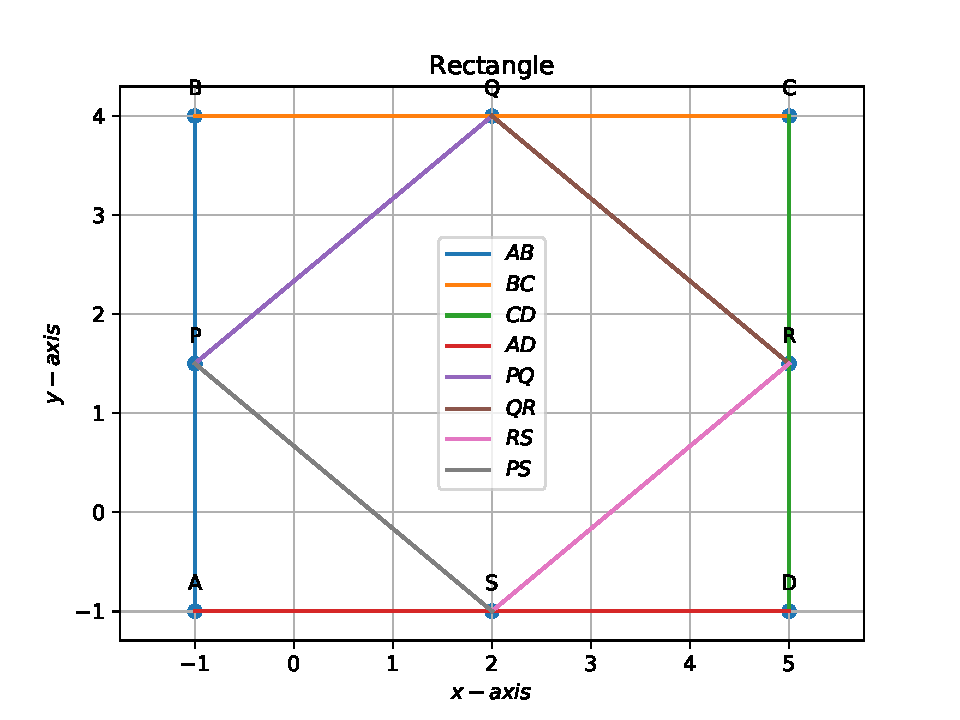
\includegraphics[width=\columnwidth]{chapters/10/7/4/8/figs/problem1.pdf}
	\end{center}
\caption{}
\label{fig:10/7/4/8Fig3}
\end{figure}
We know that PQRS is a parallelogram. To know, if it is a rectangle, we need to ascertain whether any of the two adjacent sides are perpendicular. 
That means $\brak{\vec{Q}-\vec{P}}^\top\brak{\vec{R}-\vec{Q}}$ should be equal to zero. 
\begin{align}
\vec{Q}-\vec{P} &=  \myvec{
 2 \\
 4 \\
 } - \myvec{
 -1 \\
 \frac{3}{2} \\
 } = \myvec{
 3 \\
 \frac{5}{2} \\ 
 } \\
 \vec{R}-\vec{Q} &=  \myvec{
 5 \\
 \frac{3}{2}\\
 } - \myvec{
 2 \\
 4 \\
 } = \myvec{
 3 \\
 -\frac{5}{2} \\ 
 } \\ 
 \brak{\vec{Q}-\vec{P}}^\top\brak{\vec{R}-\vec{Q}} &= \myvec{
 3 & \frac{5}{2}} \myvec{
 3 \\
 -\frac{5}{2} 
 } \neq 0
\end{align}
Therefore PQRS is not a rectangle. Let us check if it is a rhombus. For a rhombus, the diagonals bisect perpendicularly. That means $\brak{\vec{R}-\vec{P}}^\top\brak{\vec{S}-\vec{Q}}$ should be equal to zero. 
\begin{align}
\vec{R}-\vec{P} &=  \myvec{
 5 \\
 \frac{3}{2} \\
 } - \myvec{
 -1 \\
 \frac{3}{2} \\
 } = \myvec{
 6 \\
 0 \\ 
 } \\
 \vec{S}-\vec{Q} &=  \myvec{
 2 \\
 -1 \\
 } - \myvec{
 2 \\
 4 \\
 } = \myvec{
 0 \\
 -5 \\ 
 } \\ 
 \brak{\vec{R}-\vec{P}}^\top\brak{\vec{S}-\vec{Q}} &= \myvec{
 6 & 0} \myvec{
 0 \\
 -5 \\
 } = 0
\end{align}
Therefore $PQRS$ is a rhombus.


\item Without using the Baudhayana theorem, show that the points $(4,4),(3,5)$ and $(-1,-1)$ are the vertices of a right angled triangle.
\label{chapters/11/10/1/6}
\iffalse
\documentclass[journal,12pt,twocolumn]{IEEEtran}
\usepackage[none]{hyphenat}
\usepackage{graphicx}
\usepackage{listings}
\usepackage[english]{babel}
\usepackage{graphicx}
\usepackage{caption} 
\usepackage{amsmath}
\usepackage{hyperref}
\usepackage{booktabs}
\usepackage{array}


\title{\textbf{\\Assignment on line}}
\author{Sireesha Abbavaram - FWC22060}
\begin{document}
\maketitle


\section{Question}
\textbf{\textit{Class 11, Exercise 10.1, Q(6):}
\fi
	\begin{figure}[!ht]
		\centering
 \includegraphics[width=\columnwidth]{chapters/11/10/1/6/figs/triangle.png}
		\caption{}
		\label{fig:11/10/1/6}
  	\end{figure}
\iffalse
}

\begin{figure}[h!]
\centering
\includegraphics[scale=0.35]{triangle.png}
\centering
\caption{Traingle ABC}
\end{figure}


\section{Solution}
\raggedright 
\vspace{0.25cm}
Let A,B and C be the vertices of a given traingle with coordinates $\myvec{
4 \\
4
}
, \myvec{
3 \\
5
}
 and \myvec{
-1 \\
-1
} $
\raggedright
. we have verify whther the given vertices are of right angled triangle or not.\\
\begin{center}
\raggedright
Let The directional vector of two vectors A and B is given as AB (m1)=A-B.
\end{center}
\vspace{0.25cm}
\begin{center}
The directional vector of the vectors B and C is given as BC (m2)=B-C.
\end{center}
\vspace{0.25cm}
\begin{center}
The directinal vector of the vectors C and A is given as CA (m3)=C-A.
\end{center}
\vspace{0.25cm}
The angle between any two vectors is given by
\boldmath
\\ $ cos b =\frac{(m1)^T(m2)}{||m1|| ||m2||}  equation-1$
\unboldmath
\vspace{0.5cm}\raggedright\\
Where b is the angle between the two vectors .
when the angle b=90 ,we get cos 90=0.
\vspace{0.5cm}\raggedright\\
It implies that the numerator of the equation 1 should be zero.

\vspace{0.25cm}
 In order to prove that the triangle is right angled we have to show any two vectors should be orthogonal to each other.
 
\vspace{0.25cm}\raggedright
So we need to show $(A-B)^T(B-C) or (B-C)^T(C-A) or (C-A)^T(A-B) $ is equal to zero.
\fi

\vspace{0.5cm}\raggedright
\begin{align}
	\vec{C}-\vec{A}&=\myvec{
-5 \\
	-5},
\\
	\vec{A}-\vec{B}&=\myvec{
1 \\
-1 
}
\\
	\implies \brak{\vec{C}-\vec{A}}^{\top}
	\brak{\vec{A}-\vec{B}}&=0
\end{align}
Thus, $AB \perp AC$.
\iffalse
\vspace{0.25cm}\raggedright
Thus we have right angle at the vertex A.


\vspace{0.2cm}
\section*{Construction}
\centering
\vspace{0.2cm}
{
\setlength\extrarowheight{2pt}
\begin{tabular}{|c|c|c|}
	\hline
	\textbf{Symbol}&\textbf{Value}&\textbf{Description}\\
	\hline
	A & (4,4) & Vertex A\\
	\hline
	B & (3,5) & Vertex B\\
	\hline
	C & (-1,-1) & Vertex C\\
	\hline
	
\end{tabular}
}

\vspace{0.6cm}
Get the python code of the figures from
\begin{table}[h]
\large
\centering
\begin{tabular}{|l|}
\hline
https://github.com/Sireesha1602/sireesha/
\\blob/main/line assignment \\
\hline
\end{tabular}

\end{table}




\end{document}
\fi

\item The line through the points $(h, 3)$ and $(4, 1)$ intersects the line $7x- 9y- 19= 0$ at right angle. Find the value of $h$.
\label{chapters/11/10/3/10}
\\
\solution
\iffalse
\documentclass[12pt]{article}
\usepackage{graphicx}
\usepackage[none]{hyphenat}
\usepackage{graphicx}
\usepackage{listings}
\usepackage[english]{babel}
\usepackage{graphicx}
\usepackage{caption} 
\usepackage{booktabs}
\usepackage{array}
\usepackage{amssymb} % for \because
\usepackage{amsmath}   % for having text in math mode
\usepackage{extarrows} % for Row operations arrows
\usepackage{listings}
\usepackage[utf8]{inputenc}
\lstset{
  frame=single,
  breaklines=true
}
\usepackage{hyperref}
  
%Following 2 lines were added to remove the blank page at the beginning
\usepackage{atbegshi}% http://ctan.org/pkg/atbegshi
\AtBeginDocument{\AtBeginShipoutNext{\AtBeginShipoutDiscard}}


%New macro definitions
\newcommand{\mydet}[1]{\ensuremath{\begin{vmatrix}#1\end{vmatrix}}}
\providecommand{\brak}[1]{\ensuremath{\left(#1\right)}}
\newcommand{\solution}{\noindent \textbf{Solution: }}
\newcommand{\myvec}[1]{\ensuremath{\begin{pmatrix}#1\end{pmatrix}}}
\providecommand{\norm}[1]{\left\lVert#1\right\rVert}
\providecommand{\abs}[1]{\left\vert#1\right\vert}
\let\vec\mathbf

\begin{document}

\begin{center}
\title{\textbf{LINE}}
\date{\vspace{-5ex}} %Not to print date automatically
\maketitle
\end{center}

\section{11$^{th}$ Maths - EXERCISE-10.3}
\begin{enumerate}
\end{enumerate}
\section{SOLUTION}
\fi
Let
Given points are 
\begin{align}
\vec{A}=\myvec{h\\ 3},\vec{B}=\myvec{4\\ 1} 
\implies \vec{B}-\vec{A}=
\myvec{4-h\\ -2}
\end{align}
The given line equation  can be expressed as
\begin{align}
\myvec{7& -9}\vec{x}&=19
\end{align}
yielding 
\begin{align}
\vec{n}=\myvec{7\\ -9},
\vec{m}=\myvec{9\\ 7}
\end{align}
Thus, 
\begin{align}
	\vec{m}^\top\brak{\vec{B}- \vec{A}}&=0\\
\implies\myvec{9& 7}\myvec{4-h\\ -2}&=0\\
\implies h&=\frac{22}{9}
\end{align}
See Fig. 
		\ref{fig:chapters/11/10/3/10/Figure}.
\begin{figure}[h]
\centering
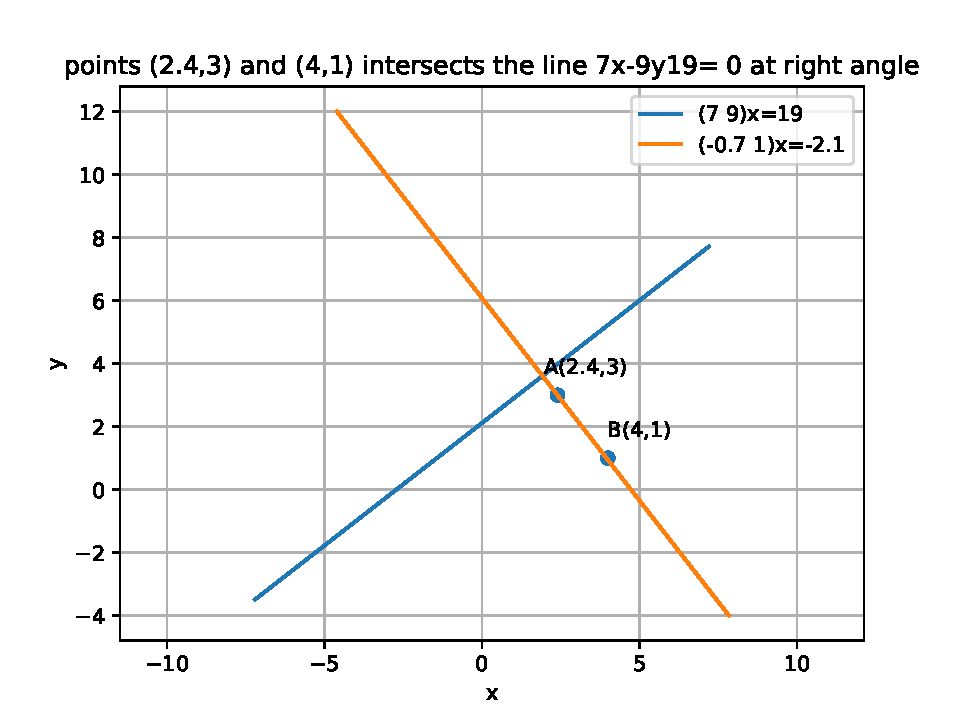
\includegraphics[width=\columnwidth]{chapters/11/10/3/10/figs/fig.pdf}
\caption{}
		\label{fig:chapters/11/10/3/10/Figure}
\end{figure}

\item In the following cases, determine whether the given planes are parallel or perpendicular, and in case they are neither, find the angles between them.
\begin{enumerate}
\item $7x + 5y + 6z + 30 = 0$ and $3x – y – 10z + 4 = 0$
\item $2x + y + 3z – 2 = 0$ and $x – 2y + 5 = 0$
\item $2x – 2y + 4z + 5 = 0$ and $3x – 3y + 6z – 1 = 0$
\item $2x – y + 3z – 1 = 0$ and $2x – y + 3z + 3 = 0$
\item $4x + 8y + z – 8 = 0$ and $y + z – 4 = 0$
\end{enumerate}
    \solution
		\iffalse
\documentclass[journal,12pt,twocolumn]{IEEEtran}
\usepackage{romannum}
\usepackage{float}
\usepackage{setspace}
\usepackage{gensymb}
\singlespacing
\usepackage[cmex10]{amsmath}
\usepackage{amsthm}
\usepackage{mathrsfs}
\usepackage{txfonts}
\usepackage{stfloats}
\usepackage{bm}
\usepackage{cite}
\usepackage{cases}
\usepackage{subfig}
\usepackage{longtable}
\usepackage{multirow}
\usepackage{enumitem}
\usepackage{mathtools}
\usepackage{steinmetz}
\usepackage{tikz}
\usepackage{circuitikz}
\usepackage{verbatim}
\usepackage{tfrupee}
\usepackage[breaklinks=true]{hyperref}
\usepackage{tkz-euclide}
\usetikzlibrary{calc,math}
\usepackage{listings}
    \usepackage{color}                                            %%
    \usepackage{array}                                            %%
    \usepackage{longtable}                                        %%
    \usepackage{calc}                                             %%
    \usepackage{multirow}                                         %%
    \usepackage{hhline}                                           %%
    \usepackage{ifthen}                                           %%
  %optionally (for landscape tables embedded in another document): %%
    \usepackage{lscape}     
\usepackage{multicol}
\usepackage{chngcntr}
\DeclareMathOperator*{\Res}{Res}
\renewcommand\thesection{\arabic{section}}
\renewcommand\thesubsection{\thesection.\arabic{subsection}}
\renewcommand\thesubsubsection{\thesubsection.\arabic{subsubsection}}

\renewcommand\thesectiondis{\arabic{section}}
\renewcommand\thesubsectiondis{\thesectiondis.\arabic{subsection}}
\renewcommand\thesubsubsectiondis{\thesubsectiondis.\arabic{subsubsection}}

% correct bad hyphenation here
\hyphenation{op-tical net-works semi-conduc-tor}
\def\inputGnumericTable{}                                 %%

\lstset{
frame=single, 
breaklines=true,
columns=fullflexible
}

\begin{document}


\newtheorem{theorem}{Theorem}[section]
\newtheorem{problem}{Problem}
\newtheorem{proposition}{Proposition}[section]
\newtheorem{lemma}{Lemma}[section]
\newtheorem{corollary}[theorem]{Corollary}
\newtheorem{example}{Example}[section]
\newtheorem{definition}[problem]{Definition}
\newcommand{\BEQA}{\begin{eqnarray}}
\newcommand{\EEQA}{\end{eqnarray}}
\newcommand{\define}{\stackrel{\triangle}{=}}

\bibliographystyle{IEEEtran}
\providecommand{\mbf}{\mathbf}
\providecommand{\pr}[1]{\ensuremath{\Pr\left(#1\right)}}
\providecommand{\qfunc}[1]{\ensuremath{Q\left(#1\right)}}
\providecommand{\sbrak}[1]{\ensuremath{{}\left[#1\right]}}
\providecommand{\lsbrak}[1]{\ensuremath{{}\left[#1\right.}}
\providecommand{\rsbrak}[1]{\ensuremath{{}\left.#1\right]}}
\providecommand{\brak}[1]{\ensuremath{\left(#1\right)}}
\providecommand{\lbrak}[1]{\ensuremath{\left(#1\right.}}
\providecommand{\rbrak}[1]{\ensuremath{\left.#1\right)}}
\providecommand{\cbrak}[1]{\ensuremath{\left\{#1\right\}}}
\providecommand{\lcbrak}[1]{\ensuremath{\left\{#1\right.}}
\providecommand{\rcbrak}[1]{\ensuremath{\left.#1\right\}}}
\theoremstyle{remark}
\newtheorem{rem}{Remark}
\newcommand{\sgn}{\mathop{\mathrm{sgn}}}
\providecommand{\abs}[1]{\left\vert#1\right\vert}
\providecommand{\res}[1]{\Res\displaylimits_{#1}} 
\providecommand{\norm}[1]{\left\lVert#1\right\rVert}
\providecommand{\mtx}[1]{\mathbf{#1}}
\providecommand{\mean}[1]{E\left[ #1 \right]}
\providecommand{\fourier}{\overset{\mathcal{F}}{ \rightleftharpoons}}
\providecommand{\system}{\overset{\mathcal{H}}{ \longleftrightarrow}}
\newcommand{\solution}{\noindent \textbf{Solution: }}
\newcommand{\cosec}{\,\text{cosec}\,}
\providecommand{\dec}[2]{\ensuremath{\overset{#1}{\underset{#2}{\gtrless}}}}
\newcommand{\myvec}[1]{\ensuremath{\begin{pmatrix}#1\end{pmatrix}}}
\newcommand{\mydet}[1]{\ensuremath{\begin{vmatrix}#1\end{vmatrix}}}
\numberwithin{equation}{subsection}
\makeatletter
\@addtoreset{figure}{problem}
\makeatother

\let\StandardTheFigure\thefigure
\let\vec\mathbf
\renewcommand{\thefigure}{\theproblem}



\def\putbox#1#2#3{\makebox[0in][l]{\makebox[#1][l]{}\raisebox{\baselineskip}[0in][0in]{\raisebox{#2}[0in][0in]{#3}}}}
     \def\rightbox#1{\makebox[0in][r]{#1}}
     \def\centbox#1{\makebox[0in]{#1}}
     \def\topbox#1{\raisebox{-\baselineskip}[0in][0in]{#1}}
     \def\midbox#1{\raisebox{-0.5\baselineskip}[0in][0in]{#1}}

\vspace{3cm}


\title{Assignment 1}
\author{Jaswanth Chowdary Madala}





% make the title area
\maketitle

\newpage

%\tableofcontents

\bigskip

\renewcommand{\thefigure}{\theenumi}
\renewcommand{\thetable}{\theenumi}

\begin{enumerate}

\textbf{Solution:} 
\fi
		The angle between the planes is the angle between the normals of the given planes.
\begin{align}
\vec{n_1}^{\top}\vec{x} = c_1, \, \vec{n_2}^{\top}\vec{x} &= c_2
\end{align}
The angle $\theta$ between the planes is given by,
\begin{align}
\cos{\theta} &= \frac{\vec{n_1}^{\top}\vec{n_2}}{\norm{\vec{n_1}}\norm{\vec{n_2}}}
\end{align}

\begin{enumerate}
\item
\begin{align}
\vec{n_1} = \myvec{7\\5\\6}, \, \vec{n_2} &= \myvec{3\\-1\\-10}\\
\implies \vec{n_1}^{\top}\vec{n_2} = \myvec{7&5&6}\myvec{3\\-1\\-10}
	&= -44\\
\norm{\vec{n_1}} = \sqrt{7^2+5^2+6^2}
&= \sqrt{110}\\
\norm{\vec{n_2}} = \sqrt{3^2+\brak{-1}^2+\brak{-10}^2} 
&= \sqrt{110}\\
\cos{\theta} = -\frac{44}{\sqrt{110}\sqrt{110}}
&= -\frac{2}{5}
\end{align}
The planes are inclined at an angle of $\arccos\brak{{-\frac{2}{5}}}$ degrees.

\item
\begin{align}
\vec{n_1} = \myvec{2\\1\\3},\, \vec{n_2} &= \myvec{1\\-2\\0}\\
\vec{n_1}^{\top}\vec{n_2} = \myvec{2&1&3}\myvec{1\\-2\\0}\\
= 0
\end{align}  
The planes are perpendicular.
\item
\begin{align}
\vec{n_1} = \myvec{2\\-2\\4},\, \vec{n_2} &= \myvec{3\\-3\\6}\\
\vec{n_1}^{\top}\vec{n_2} = \myvec{2&-2&4}\myvec{3\\-3\\6}
&= 36\\
\norm{\vec{n_1}} = \sqrt{2^2+\brak{-2}^2+4^2}
&= \sqrt{24}\\
\norm{\vec{n_2}} = \sqrt{3^2+\brak{-3}^2+6^2} 
&= \sqrt{54}\\
\cos{\theta}= \frac{36}{\sqrt{24}\sqrt{54}}\\
&= 1
\end{align}
The planes are parallel.
\item
\begin{align}
\vec{n_1} = \myvec{2\\-1\\3}, \, \vec{n_2} &= \myvec{2\\-1\\3}\\
\vec{n_1}^{\top}\vec{n_2} = \myvec{2&-1&3}\myvec{2\\-1\\3}
&= 14\\
\norm{\vec{n_1}} &= \sqrt{2^2+\brak{-1}^2+3^2}
&= \sqrt{14}\\
\norm{\vec{n_2}} = \sqrt{2^2+\brak{-1}^2+3^2}
&= \sqrt{14}\\
\cos{\theta} = \frac{14}{\sqrt{14}\sqrt{14}}
&= 1
\end{align}
The planes are parallel.
\item
\begin{align}
\vec{n_1} = \myvec{4\\8\\1}, \, \vec{n_2} &= \myvec{0\\1\\1}\\
\vec{n_1}^{\top}\vec{n_2} = \myvec{4&8&1}\myvec{0\\1\\1}
&= 9\\
\norm{\vec{n_1}} = \sqrt{4^2+8^2+1^2}
&= 9\\
\norm{\vec{n_2}} = \sqrt{0^2+1^2+1^2} 
&= \sqrt{2}\\
\cos{\theta} = \frac{9}{9\sqrt{2}}
&= \frac{1}{\sqrt{2}}
\end{align}
The planes are inclined at an angle of 45 degrees.
\end{enumerate}

		\item 
 Show that the line joining the origin to the point $(2, 1, 1)$ is perpendicular to the
line determined by the points $(3, 5, – 1), (4, 3, – 1)$.
\\
    \solution
		\iffalse
\documentclass[12pt]{article}
\usepackage{graphicx}
\usepackage{amsmath}
\usepackage{mathtools}
\usepackage{gensymb}
\usepackage[utf8]{inputenc}
\usepackage{float}
\newcommand{\mydet}[1]{\ensuremath{\begin{vmatrix}#1\end{vmatrix}}}
\providecommand{\brak}[1]{\ensuremath{\left(#1\right)}}
\providecommand{\norm}[1]{\left\lVert#1\right\rVert}
\newcommand{\solution}{\noindent \textbf{Solution: }}
\newcommand{\myvec}[1]{\ensuremath{\begin{pmatrix}#1\end{pmatrix}}}
\let\vec\mathbf

\begin{document}
\begin{center}
\textbf\large{CLASS-12 \\ CHAPTER-11 \\ THREE DIMENSIONAL GEOMETRY}
\end{center}
\section*{Excercise 11.4}

\\
\solution
\\
\fi
Let
\begin{align}
  \vec{P}=\myvec{2\\1\\1},\vec{A}=\myvec{3\\5\\-1},\vec{B}=\myvec{4\\3\\-1}
\end{align}
Then
		\begin{align}
	\vec{m}=\vec{A}-\vec{B}=\myvec{-1\\2\\0}
		\end{align}
		and
		\begin{align}
			\vec{m}^\top\vec{P}=
			\myvec{-1&2&0}\myvec{2\\1\\1}=0
		\end{align}
		This proves the result.


	\item  If $l_1, m_1,n_1 \text{ and } l_2,m_2,n_2$ are the direction cosines of two mutually perpendicular lines, show that the direction cosines of the line perpendicular to both these are  $m_1n_2-m_2n_1,n_1l_2-n_2l_1,l_1m_2-l_2m_1$.
\\
    \solution
		\iffalse
\documentclass[12pt]{article}
\setlength{\textwidth}{5cm}
\paperheight 12in
\paperwidth 12in
\usepackage{graphicx}
\usepackage[margin=0.2in]{geometry}
\usepackage{amsmath}
\usepackage{array}
\usepackage{booktabs}
\usepackage{listings}
\providecommand{\norm}[1]{\left\lVert#1\right\rVert}
\providecommand{\abs}[1]{\left\vert#1\right\vert}
\setlength{\arraycolsep}{2.5pt} % default: 5pt
\medmuskip = 1mu % default: 4mu plus 2mu minus 4mu
\usepackage{enumerate}
\let\vec\mathbf
\newcommand{\myvec}[1]{\ensuremath{\begin{pmatrix}#1\end{pmatrix}}}
\newcommand{\mydet}[1]{\ensuremath{\begin{vmatrix}#1\end{vmatrix}}}
\providecommand{\brak}[1]{\ensuremath{\left(#1\right)}}
\lstset{
frame=single,
breaklines=true,
columns=fullflexible
}
\title{\textbf{Line Assignment}}
\author{Srikanth}
\date{January 2023}
\begin{document}
\maketitle
\paragraph{\textit{Problem Statement} -
\section*{Solution}
\fi
Let 
\begin{align}
 \vec{A}=\myvec{l_1\\m_1\\n_1},\,\vec{B}=\myvec{l_2\\m_2\\n_2}, \,
 \vec{C}&=\myvec{m_1n_2-m_2n_1\\n_1l_2-n_2l_1\\l_1m_2-l_2m_1}.
 \end{align}
 Given that 
 \begin{align} 
 \vec{A}^{\top}\vec{B}=\vec{0},\, 
  \vec{A}^{\top}\vec{A}=\vec{1},\,
   \vec{B}^{\top}\vec{B}=\vec{1} 
 \end{align}
 Let 
\begin{align}
\vec{P}=\myvec{\vec{A} & \vec{B} & \vec{C}} 
	=\myvec{
l_1&l_2&m_1n_2-m_2n_1\\
        m_1&m_2&n_1l_2-n_2l_1\\
        n_1&n_2&l_1m_2-l_2m_1
}
	\end{align}
Then 	
	\begin{align}
	\vec{P}^{\top} \vec{P}=
%		\myvec{
%l_1^2+m_1^2+n_1^2&l_1l_2+m_1m_2+n_1n_2&l_1(m_1n_2-m_2n_1)+m_1(n_1l_2-n_2l_1)+n_1(l_1m_2-l_2m_1)\\
%l_1l_2+m_1n_2+n_1n_2&l_2^2+m_2^2+n_2^2&l_2(m_1n_2-m_2n_1)+m_2(n_1l_2-n_2l_1)+n_2(l_1m_2-l_2m_1)\\
%l_1(m_1n_2-n_2m_1)+m_1(n_1l_2-n_2l_1)\\+n_1(l_1m_2-l_2m_1)&l_2(m_1n_2-m_2n_1)+m_2(n_1l_2-n_2l_1)+n_2(l_1m_2-l_2m_1)&(l_1m_2-l_2m_1)^2+(n_1l_2-n_2l_1)^2+(m_1n_2-m_2n_1)^2
%}
\vec{I}
	\end{align}
	Hence, the three vectors are mutually perpendicular.

	\item If the lines $\frac{x-1}{-3} = \frac{y-2}{2k} = \frac{z-3}{2}$ and  $\frac{x-1}{3k} = \frac{y-1}{1} = \frac{z-6}{-5}$ are perpendicular, find the value of k.\\
    \solution
		\iffalse
\documentclass[A4,12pt,twocolumn]{IEEEtran}
%
\usepackage{setspace}
\usepackage{gensymb}
%\doublespacing
\singlespacing

%\usepackage{graphicx}
%\usepackage{amssymb}
%\usepackage{relsize}
\usepackage[cmex10]{amsmath}
%\usepackage{amsthm}
%\interdisplaylinepenalty=2500
%\savesymbol{iint}
%\usepackage{txfonts}
%\restoresymbol{TXF}{iint}
%\usepackage{wasysym}
\usepackage{amsthm}
%\usepackage{iithtlc}
\usepackage{mathrsfs}
\usepackage{txfonts}
\usepackage{stfloats}
\usepackage{bm}
\usepackage{cite}
\usepackage{cases}
\usepackage{subfig}
%\usepackage{xtab}
\usepackage{longtable}
\usepackage{multirow}
%\usepackage{algorithm}
%\usepackage{algpseudocode}
\usepackage{enumitem}
\usepackage{mathtools}
\usepackage{steinmetz}
\usepackage{tikz}
\usepackage{circuitikz}
\usepackage{verbatim}
\usepackage{tfrupee}
\usepackage[breaklinks=true]{hyperref}
%\usepackage{stmaryrd}
\usepackage{tkz-euclide} % loads  TikZ and tkz-base
%\usetkzobj{all}
\usetikzlibrary{calc,math}
\usepackage{listings}
    \usepackage{color}                                            %%
    \usepackage{array}                                            %%
    \usepackage{longtable}                                        %%
    \usepackage{calc}                                             %%
    \usepackage{multirow}                                         %%
    \usepackage{hhline}                                           %%
    \usepackage{ifthen}                                           %%
  %optionally (for landscape tables embedded in another document): %%
    \usepackage{lscape}     
\usepackage{multicol}
\usepackage{chngcntr}
%\usepackage{enumerate}

%\usepackage{wasysym}
%\newcounter{MYtempeqncnt}
\DeclareMathOperator*{\Res}{Res}
%\renewcommand{\baselinestretch}{2}
\renewcommand\thesection{\arabic{section}}
\renewcommand\thesubsection{\thesection.\arabic{subsection}}
\renewcommand\thesubsubsection{\thesubsection.\arabic{subsubsection}}

\renewcommand\thesectiondis{\arabic{section}}
\renewcommand\thesubsectiondis{\thesectiondis.\arabic{subsection}}
\renewcommand\thesubsubsectiondis{\thesubsectiondis.\arabic{subsubsection}}

% correct bad hyphenation here
\hyphenation{op-tical net-works semi-conduc-tor}
\def\inputGnumericTable{}                                 %%

\lstset{
%language=C,
frame=single, 
breaklines=true,
columns=fullflexible
}
%\lstset{
%language=tex,
%frame=single, 
%breaklines=true
%}

\begin{document}
%


\newtheorem{theorem}{Theorem}[section]
\newtheorem{problem}{Problem}
\newtheorem{proposition}{Proposition}[section]
\newtheorem{lemma}{Lemma}[section]
\newtheorem{corollary}[theorem]{Corollary}
\newtheorem{example}{Example}[section]
\newtheorem{definition}[problem]{Definition}
%\newtheorem{thm}{Theorem}[section] 
%\newtheorem{defn}[thm]{Definition}
%\newtheorem{algorithm}{Algorithm}[section]
%\newtheorem{cor}{Corollary}
\newcommand{\BEQA}{\begin{eqnarray}}
\newcommand{\EEQA}{\end{eqnarray}}
\newcommand{\define}{\stackrel{\triangle}{=}}

\bibliographystyle{IEEEtran}
%\bibliographystyle{ieeetr}


\providecommand{\mbf}{\mathbf}
\providecommand{\pr}[1]{\ensuremath{\Pr\left(#1\right)}}
\providecommand{\qfunc}[1]{\ensuremath{Q\left(#1\right)}}
\providecommand{\sbrak}[1]{\ensuremath{{}\left[#1\right]}}
\providecommand{\lsbrak}[1]{\ensuremath{{}\left[#1\right.}}
\providecommand{\rsbrak}[1]{\ensuremath{{}\left.#1\right]}}
\providecommand{\brak}[1]{\ensuremath{\left(#1\right)}}
\providecommand{\lbrak}[1]{\ensuremath{\left(#1\right.}}
\providecommand{\rbrak}[1]{\ensuremath{\left.#1\right)}}
\providecommand{\cbrak}[1]{\ensuremath{\left\{#1\right\}}}
\providecommand{\lcbrak}[1]{\ensuremath{\left\{#1\right.}}
\providecommand{\rcbrak}[1]{\ensuremath{\left.#1\right\}}}
\theoremstyle{remark}
\newtheorem{rem}{Remark}
\newcommand{\sgn}{\mathop{\mathrm{sgn}}}
\providecommand{\abs}[1]{\left\vert#1\right\vert}
\providecommand{\res}[1]{\Res\displaylimits_{#1}} 
\providecommand{\norm}[1]{\left\lVert#1\right\rVert}
%\providecommand{\norm}[1]{\lVert#1\rVert}
\providecommand{\mtx}[1]{\mathbf{#1}}
\providecommand{\mean}[1]{E\left[ #1 \right]}
\providecommand{\fourier}{\overset{\mathcal{F}}{ \rightleftharpoons}}
%\providecommand{\hilbert}{\overset{\mathcal{H}}{ \rightleftharpoons}}
\providecommand{\system}{\overset{\mathcal{H}}{ \longleftrightarrow}}
	%\newcommand{\solution}[2]{\textbf{Solution:}{#1}}
\newcommand{\solution}{\noindent \textbf{Solution: }}
\newcommand{\cosec}{\,\text{cosec}\,}
\providecommand{\dec}[2]{\ensuremath{\overset{#1}{\underset{#2}{\gtrless}}}}
\newcommand{\myvec}[1]{\ensuremath{\begin{pmatrix}#1\end{pmatrix}}}
\newcommand{\mydet}[1]{\ensuremath{\begin{vmatrix}#1\end{vmatrix}}}
%\numberwithin{equation}{section}
\numberwithin{equation}{subsection}
%\numberwithin{problem}{section}
%\numberwithin{definition}{section}
\makeatletter
\@addtoreset{figure}{problem}
\makeatother

\let\StandardTheFigure\thefigure
\let\vec\mathbf
%\renewcommand{\thefigure}{\theproblem.\arabic{figure}}
\renewcommand{\thefigure}{\theproblem}
%\setlist[enumerate,1]{before=\renewcommand\theequation{\theenumi.\arabic{equation}}
%\counterwithin{equation}{enumi}


%\renewcommand{\theequation}{\arabic{subsection}.\arabic{equation}}

\def\putbox#1#2#3{\makebox[0in][l]{\makebox[#1][l]{}\raisebox{\baselineskip}[0in][0in]{\raisebox{#2}[0in][0in]{#3}}}}
     \def\rightbox#1{\makebox[0in][r]{#1}}
     \def\centbox#1{\makebox[0in]{#1}}
     \def\topbox#1{\raisebox{-\baselineskip}[0in][0in]{#1}}
     \def\midbox#1{\raisebox{-0.5\baselineskip}[0in][0in]{#1}}

\vspace{3cm}


\title{ASSIGNMENT}
\author{Shristy Sharma (EE22BNITS11001)}





% make the title area
\maketitle

\newpage

%\tableofcontents

\bigskip

\renewcommand{\thefigure}{\theenumi}
\renewcommand{\thetable}{\theenumi}
%\renewcommand{\theequation}{\theenumi}


%Download all python codes 
%
%\begin{lstlisting}
%svn co https://github.com/JayatiD93/trunk/My_solution_design/codes
%\end{lstlisting}

%Download all and latex-tikz codes from 
%
%\begin{lstlisting}
%svn co https://github.com/gadepall/school/trunk/ncert/geometry/figs
%\end{lstlisting}
%


\section{PROBLEM }
\section{SOLUTION:}
\fi
From the given information,
\begin{align}
\vec{m}_1 = \myvec{-3\\ 2k\\ 2},\,  \vec{m}_2 =\myvec{3k\\ 1\\ -5} 
	\implies \myvec{-3& 2k& 2}^{\top} \myvec{3k\\ 1\\ -5} &=0
	\\
	\implies k &= -\frac{10}{7}
\end{align}
See Fig. 
\begin{figure}[h!]
  \centering
   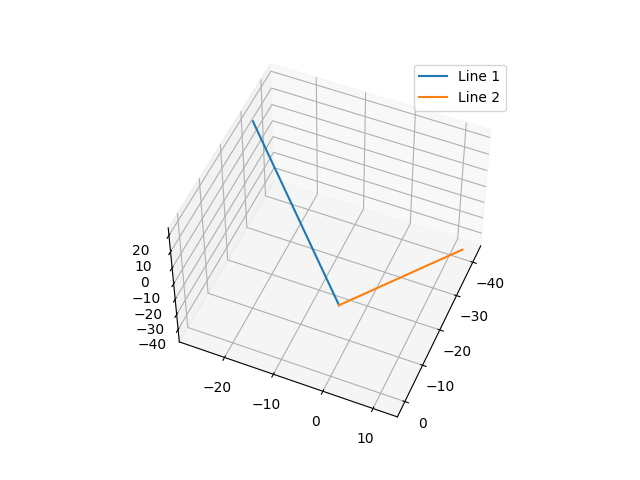
\includegraphics[width=\columnwidth]{chapters/12/11/4/6/figs/line_1.png}
    \caption{lines represented for the given points and direction vector with k=$\frac{-10}{7}$}
     \label{fig:chapters/12/11/4/6/1}
     \end{figure}  



\item If $\vec{a},\vec{b},\vec{c}$ are mutually perpendicular vectors of equal magnitudes, show that the vector $\vec{c}.\vec{d}$=15 is equally inclined to $\vec{a},\vec{b}$ and $\vec{c}$.\\
\end{enumerate}
